\documentclass[14pt,a4paper]{extarticle}

\usepackage{geometry}
\geometry{left=30mm,right=15mm,top=20mm,bottom=20mm}
\usepackage{fontspec}
\usepackage{polyglossia}
\setmainlanguage{russian}
\setotherlanguage{english}
\setmainfont{Times New Roman}
\newfontfamily\cyrillicfont{Times New Roman}
\setmonofont{Courier New}
\newfontfamily\cyrillicfonttt{Courier New}
\usepackage{indentfirst}
\usepackage{graphicx}
\usepackage{float}
\usepackage{caption}
\usepackage{amsmath,amssymb}
\usepackage{csquotes}
\usepackage[
    backend=biber,
    bibencoding=utf8,
    sorting=none,
    style=gost-numeric,
    language=autobib,
    autolang=other,
    clearlang=true,
    defernumbers=false,
    sortcites=true,
    doi=false,
    isbn=false,
]{biblatex}
\addbibresource{/Users/gk/Code/super-duper-disser/itmo-phd-thesis-template-en/biblio/references.bib}
\addbibresource{/Users/gk/Code/super-duper-disser/itmo-phd-thesis-template-en/biblio/own.bib}

\setlength{\parindent}{1.25cm}
\setlength{\parskip}{0pt}
\linespread{1.15}
\emergencystretch=3em
\sloppy

\begin{document}

\begin{center}
\textbf{Введение}
\end{center}

\paragraph*{Актуальность темы исследования.}

Российская система территориального планирования связывает доступность объектов обслуживания с показателями национальных программ и проектов. Национальная цель по достижению комфортной и безопасной среды для жизни, поставлена в указе Президента РФ №309 от 7 мая 2024 года \cite{rfDecree309_2024}. Национальные направления развития выражаются в федеральных проектах, в частности, в проекте по формированию комфортной городской среды \cite{federalProjectFkgsPassport}. Прикладную часть программы федерального уровня реализовывают региональная программы, которые задают уже тот уровень, на котором локальный исполнительный орган власти непосредственно отвечает за достижение целевых показателей  эффективности \cite{spbRegionalFkgs}.

Несоответствие заключается в том, что оценки доступности и обеспеченности по нормативам отвечают на вопрос, где и что должно быть размещено, а ПКРТИ отвечает на вопрос, как развивать дорожно-транспортную инфраструктуру. В случае, если эти решения готовятся последовательно, возникает риск создания неэффективного плана застройки территории объектами обслуживания населения, поскольку согласование транспортного плана будет происходить на последующих этапах.

Задача обеспечения доступности объектов предложения не нова. Изначально, города строились с ориентацией на пешеходной движение, затем, с появлением всё новых видов мобильности, городская топология подстраивалась под них. Так, с увеличением расстояний и спроса на личный транспорт, городское пространство стало менее человеко-ориентированным, и, как следствие, менее доступным.

\paragraph*{Степень разработанности проблемы.}

Классическая линия моделей оптимального размещения объектов формализовала обслуживание как выбор узлов или площадок при заданном спросе и заданной сети расстояний. Задача размещения складов задала базовую постановку выбора складов с учетом затрат обслуживания спроса \cite{kuehn1963warehouse}. P-медиана и p-центр закрепили две ключевые логики: минимизацию суммарного расстояния и ограничение худшего расстояния до объекта \cite{hakimi1964medians}. Для общественных сервисов важным развитием стали покрывающие постановки. Покрытие множества минимизирует число объектов, достаточных для покрытия спроса в пределах нормативного расстояния \cite{toregas1971emergency}. Максимальное покрытие максимизирует покрытый спрос при ограниченном числе объектов \cite{church1974mclp}. В этих и других моделях оптимального размещения транспортная сеть обычно выражена фиксированной матрицей расстояний или времен, а не как самостоятельный объект решения.

Класс задач совместного размещения объектов и проектирования сети включает в себя одновременный выбор мест размещения объектов обслуживания и изменения транспортных связей  \cite{daskin1993towardIntegrated} \cite{melkote1996integrated}. Решение задач покрытия в такой постановке показывает, что удовлетворение спроса зависит от изменений в сети \cite{melkote1998maximumCovering}. Решение этой задачи было также рассмотрено с учетом ограничения на вместимость входящих потоков и различной стоимостью добавления ребер в сети \cite{melkote2000capacitated}. Таким образом, совместное рассмотрение задачи оптимального размещения объектов и моделирования изменений сети был выделено в отдельную категорию Facility-location Network Design problem (FLND)\cite{melkote2001integrated}. Необходимо отметить, что при применении оптимизации размещения объектов к задаче покрытия спроса на доступ к социальной инфраструктуре в большинстве случаев необходимо рассматривать расширенную постановку задачи Facility location с учетом вместимости объектов обслуживания и размера спроса в заданной точке пространства.

\paragraph*{Цель исследования.}
Увеличение эффективности размещения объектов обслуживания населения в рамках процесса территориального планирования

\paragraph*{Задачи исследования.}
\begin{enumerate}
    \item Исследование системы управления территориальным планированием в задаче размещения объектов социального обслуживания населения;
    \item Разработка метода оценки транспортной доступности на основе критерия сезонной устойчивости;
    \item Разработка метода оптимизации сети в задаче оптимального размещения;
    \item Применение методов на примере агломераций Арктической зоны РФ.
\end{enumerate}

\paragraph*{Объект исследования.}
Подсистема территориального планирования в составе системы управления развитием территорий

\paragraph*{Предмет исследования.}
Методы и алгоритмы поддержки принятия решений по обеспечению транспортной доступности объектов обслуживания

\paragraph*{Научная новизна.}

Теоретическая значимость состоит в развитии теории оценки транспортной доступности за счет учета влияния внешних факторов, качества составляющих сети, учета её конфигурации и учета эффекта взаимосвязи между слоями сети. За счет предложенных расширений получается учесть как изменение состояний самой сети, так и оценить эффект от направленного изменения сети.

\paragraph*{Положения, выносимые на защиту.}
\begin{enumerate}
    \item Метод оценки транспортной доступности на основе критерия сезонной устойчивости, отличающийся применением методов сетевого анализа, обеспечивающий учет стохастической динамики многоуровневой сети. Положение соответствует пункту 2 паспорта специальности.
    \item Метод интеллектуальной поддержки принятия решений оптимального размещения объектов обслуживания, отличающийся применением оптимизации сети, обеспечивающий уменьшение необходимого количества объектов обслуживания. Положение соответствует пункту 9 паспорта специальности.
\end{enumerate}

\section*{Проблемно-классификационный анализ задачи размещения объектов обслуживания населения с учетом изменчивости транспортной доступности}

\subsection*{Нормативно-управленческая подходы к управлению транспортной доступностью}

В управленческой практике задача управления обеспечением доступности смещалась от контроля землепользования и функционального зонирования к совместному рассмотрению размещения объектов, транспортной сети и повседневных перемещений. Зонирование задает правовой механизм ограничения и распределения видов использования территории \cite{britannicaZoning}. Принцип функционального планирования закреплял разделение городских базовых функций \cite{gold1998charter}. Работа Hansen показала, что доступность влияет на формирование типа использования земли, а не только следует за ним \cite{hansen1959accessibility}.

Таким образом, совместное развитие транспорта и застройки становится всё более актуальным. Подход транзитно-ориентированного развития (TOD) делает эту координацию более предметной в пространстве, определяя фокус на развитие территорий вокруг станций и коридоров общественного транспорта \cite{worldbankTod3v}. Историческая реконструкция TOD показывает, что этот подход возник как попытка связать землепользование и общественный транспорт в единую модель развития \cite{carlton2009tod}. Однако стоит отметить, что в модели TOD развитие сконцентрировано вокруг транспортных кластеров -- больших станций метро, вокзалов. В таком случае, зона влияния ограничена пешеходной изохроной вокруг рассматриваемых транспортных узлов, что не обеспечивает достаточной гибкости для развития на уровне всего города, ведь часто эти территории уже застроены. Доступность определяется как совместная характеристика застройки и транспорта.

\subsection*{Подходы к моделированию обеспечения транспортной доступности}

С другой стороны, задача обеспечения заданного уровня доступности сильно завязана на инструментах и методах по ее измерению и моделированию. Как и различные подходы, приходящие из разных сфер, подходы в моделировании доступности объектов городской среды можно разделить на три категории: модели оптимального размещения, транспортные модели и сетевые.

Отдельная линия развития обеспечения доступности -- проектирование транспортной сети и проектирование сети с фиксированными затратами. Проектирование сети само по себе является классом оптимизационных задач \cite{magnanti1984networkDesign}. Проектирование сети с фиксированными затратами добавляет к выбору связей дискретные затраты открытия или изменения в сети \cite{powell1989networkDesign}. Алгоритмические работы по двойственному подъему показывают, что такая постановка требует специальных методов решения, а не сводится к обычному кратчайшему пути \cite{balakrishnan1989dualAscent}.

\subsection*{Дорожная сеть, климатические стрессоры и доступность}

Транспортная доступность не является постоянной характеристикой территории. В климатически зависимых регионах доступ к услугам меняется во времени: транспортные связи могут становиться недоступными, временно восстанавливаться или менять свою роль в сети. В арктических системах это особенно заметно, поскольку одни климатические процессы ухудшают работу наземной инфраструктуры, а другие временно создают новые возможности, например зимники и ледовые переправы. Поэтому задача доступности становится задачей оценки состояния сети в момент времени, а не только задачей расчета расстояния между поселением и ближайшим объектом обслуживания.

Существующие показатели транспортной доступности часто не учитывают, что в северных регионах зимой, весной или осенью часть дорог может быть труднопроходимой или закрытой, а экологические и инфраструктурные индикаторы не всегда адаптированы к экстремальным погодным режимам. Для территориального планирования это означает, что расчет доступности должен учитывать не только текущую сеть, но и долгосрочное изменение ее сезонных состояний. В этой логике транспортная сеть задается как климатически ограниченный или заданный внешней средой каркас, а доступность услуг пересчитывается на его допустимых состояниях.

\subsection*{Оптимальное размещение и постоянная матрица доступности}

На пространственное неравенство влияют как минимум три фактора: доступное жилье, качество транспортных альтернатив и связность с необходимыми объектами. Поэтому проблема размещения объектов обслуживания перестает быть только геометрической задачей выбора ближайшего объекта. Пространственное неравенство возникает там, где спрос, сервисы и транспортная сеть не согласованы. Следовательно, улучшить ситуацию можно несколькими типами вмешательств: открыть новый объект, увеличить мощность существующего объекта, улучшить связь между районами или изменить маршрутную структуру общественного транспорта.

Ограничение стандартной постановки состоит в том, что во многих работах расстояние между объектами спроса и объектами обслуживания считается постоянным. Однако в городском управлении дороги, маршруты общественного транспорта и параметры доступности меняются вследствие развития территории и транспортных реформ. Поэтому в интегрированных постановках матрица доступности может рассматриваться не только как вход для модели размещения, но и как результат сетевых изменений.

\subsection*{Сценарии спроса и морфологическое восстановление данных}

Пространственно-морфологическое моделирование задает источник сценариев изменения спроса. Если застройка меняется, то меняется не только транспортная сеть, но и распределение населения, рабочих мест и потребности в сервисах. Поэтому модели доступности должны учитывать не только изменение транспортного предложения, но и изменение спроса, который предъявляется к объектам обслуживания. В городском планировании это особенно важно для территорий нового развития, реконструкции промышленных зон и уплотнения застройки.

Для практического планирования нужны показатели морфологии кварталов: плотность застройки, площадь застройки, этажность, функциональный состав, потенциальная емкость территории. Но эти признаки часто фрагментарны: часть доступна из кадастровых или открытых данных, часть отсутствует, часть противоречива. Цифровые двойники городов позволяют интегрировать разные источники данных для планирования, моделирования и управления, но их качество ограничено полнотой и согласованностью входных атрибутов \cite{batty2018digitalTwin}.

\subsection*{Доступность в проектировании маршрутной сети}

Обсуждение размещения объектов естественно переходит к генерации маршрутной сети общественного транспорта. Алгоритмы проектирования городской транспортной сети должны оцениваться не только по вычислительной эффективности, пассажирским издержкам и операторским издержкам, но и по тому, насколько они обеспечивают равный доступ разных групп жителей к важным городским объектам. В такой постановке транспортная сеть выступает не фоном для расчета доступности, а самостоятельным проектным решением.

Задача проектирования маршрутной сети (TNDP) формулируется как выбор набора линий или маршрутов на городском графе при заданном спросе и ограничениях связности \cite{mandl1980tndp}. Современные постановки планирования линий рассматривают последовательные этапы генерации линий, выбора линий и настройки частот \cite{schmidt2024linePlanning}. Обзоры TNDP показывают, что задача остается комбинаторно сложной и обычно балансирует пассажирские и операторские издержки \cite{duranMicco2022tndpReview}. Практические модели планирования общественного транспорта также используют ограничения длины маршрутов, пересадок и покрытия спроса \cite{sahin2023linePlanning}.

\subsection*{Интермодальная доступность и пространственное неравенство}

Интермодальная доступность является историческим мостом от измерения связности к задаче совместного планирования. В такой постановке транспортная связность городской территории рассматривается как взаимная достижимость городских кварталов. В отличие от чисто топологических индексов дорожной сети, подход сравнивает время перемещения между кварталами по интермодальному графу с более простой геометрической близостью. Это позволяет выявлять территории, которые пространственно близки к остальному городу, но фактически плохо связаны общественным транспортом.

Меры снижения пространственного неравенства можно разделить на локальные, связующие и административные. Локальные меры добавляют новые сервисы в недостаточно обеспеченные территории. Связующие меры улучшают транспортную доступность между территориями. Административные меры меняют состав и логику управления агломерацией. Для задач обеспечения транспортной доступности особенно важна пара ``локальные -- связующие меры'', потому что она соответствует выбору между размещением объекта и изменением транспортной сети. Следовательно, задача обеспечения доступности не сводится к поиску новых площадок, а требует сравнения объектовых и сетевых вмешательств в единой модели.

\section*{Метод оценки транспортной доступности с учетом стохастической динамики многоуровневой сети}

\subsection*{Математическая постановка задачи оценки транспортной доступности}

В общем виде транспортная доступность рассматривается как достижимость допустимого пункта назначения из заданного пункта отправления при ограничении на время или стоимость пути. Для пункта отправления \(i\) индикатор доступности в момент времени \(t\) записывается как
\[
A_i(t)=
\begin{cases}
1, & \text{если } \min\limits_{j\in D_i} T_{ij}(t)\le S_i,\\
0, & \text{иначе},
\end{cases}
\]
где \(D_i\) --- множество допустимых пунктов назначения для пункта отправления \(i\), \(S_i\) --- допустимое время или стоимость пути, а \(T_{ij}(t)\) --- время или стоимость перемещения от \(i\) к \(j\) в текущем состоянии сети.

В качестве частного случая этой общей схемы в данной главе используется сеть, заданная внешней средой (EFN), из арктической статьи. В этой модели явно выделяются два параметра: внешний параметр среды \(T\) и внутренний параметр связности графа \(G(t)\). В статье отдельно подчеркивается, что в EFN транспортная топология меняется из-за температурно-зависимой допустимости ребер, а сервисная доступность меняется из-за переназначения потоков между пунктами отправления и назначения поверх допустимой сети.

\subsection*{Модель транспортной сети в условиях внешних факторов}

Исследования климатически чувствительных транспортных систем показывают, что доступность не может рассматриваться как свойство фиксированного графа. В северных регионах состояние сети определяется температурой, состоянием мерзлоты и ледовой обстановкой; сокращение периода устойчивых морозов уменьшает время эксплуатации зимних дорог, а деградация мерзлоты ведет к просадке грунта, деформации дорожного полотна и взлетно-посадочной инфраструктуры \cite{dong2025iceRoads,waite2023arcticTransport,stephenson2011arcticAccess,povoroznyuk2022arcticRoads}.

Из этого следует, что транспортная и сервисная доступность должны рассчитываться по реализованному состоянию сети, а не по постоянной матрице расстояний. В работах по доступности критически важных объектов и транспортной устойчивости сначала определяется, какие ребра остаются допустимыми после внешнего воздействия, и только затем на полученном графе оценивается достижимость нужного объекта \cite{gangwal2023criticalFacility,yin2023transportResilience}.

\subsection*{Метод оценки сезонной устойчивости транспортной доступности}

Метод оценки сезонной устойчивости транспортной доступности строится как последовательность расчетов, в которых сеть сначала приводится к допустимому состоянию для заданного момента времени, а затем на этой сети оценивается достижимость услуг, стабильность поставщиков и длительность нарушений. В отличие от статической оценки доступности, здесь интерес представляет не только значение показателя в один момент, но и то, как оно изменяется между состояниями сети.

Таким образом, метод оценки сезонной устойчивости не сводится к одной сетевой метрике. Он объединяет динамический граф, правила допустимости ребер, нормативы сервисной доступности и показатели устойчивости потоков. Это позволяет анализировать не только исчезновение связей, но и более слабые формы нарушения доступности: смену поставщика, сокращение зоны обслуживания, рост времени пути и временную изоляцию узлов.

\section*{Метод интеллектуальной поддержки принятия решений оптимального размещения объектов обслуживания на основе оптимизации транспортной сети}

\subsection*{Интегрированная задача размещения и дорожного строительства}

В работах \cite{daskin1993towardIntegrated,melkote1996integrated,melkote2001integrated} рассматривается смешанно-целочисленная постановка неемкостной задачи совместного размещения объектов и моделирования сети.

Задача состоит в выборе открываемых объектов и добавляемых ребер так, чтобы максимизировать обслуженный спрос с учетом затрат на размещение и изменение сети. В этой постановке транспортная сеть уже не является только входной матрицей расстояний: часть сетевых ребер выбирается как управляемое решение.

\subsection*{Размещение объектов при изменении транспортной доступности}

Объединяются изменения транспортной связности и размещение дополнительных сервисов, которые ранее рассматривались отдельно. Проверяемая гипотеза: улучшение связности между районами не более чем на 40\% может уменьшить минимальное число новых поликлиник, которые необходимо оптимально разместить \cite{kontsevik2024connectivityPlacement}.

Для экспериментальной постановки выбран сервис ``поликлиника''. MCLP дает решения для максимизации покрытия спроса. Используется улучшенная версия MCLP --- CLSCP-SO (Capacitated Location Set Covering Problem--System Optimal), учитывающая спрос и емкость сервисов. CLSCP-SO работает с матрицей стоимости как с постоянной. Здесь матрица стоимости является матрицей доступности между выбранными районами и оптимизируется относительно числа размещаемых поликлиник \cite{churchMurray2018,spoptLscpCapacity,kontsevik2024connectivityPlacement}.

\subsection*{Маршрутное проектирование как продолжение транспортной постановки}

Маршрутное проектирование рассматривается как Transit Network Design Problem (TNDP): требуется определить допустимый набор линий общественного транспорта, обеспечивающий удобные поездки для пассажиров при минимизации операторских затрат \cite{mandl1980tndp,duranMicco2022tndpReview,sahin2023linePlanning,morozov2026oneRuleTndp}. Инфраструктурная сеть представляется графом, где узлы соответствуют остановкам, а ребра --- физическим или временным связям между ними, взвешенным расстоянием или временем движения.

Разные стратегии генерации маршрутов сравниваются в единой формулировке TNDP. Все кандидатные решения представлены как допустимые наборы маршрутов на одном городском графе и подчиняются одинаковым ограничениям на длину маршрута и связность. Каждое решение оценивается составной целевой функцией, включающей passenger cost \(C_p\), operator cost \(C_o\), demand-weighted transport connectivity \(C_w\) и штрафы за недопустимость \cite{morozov2026oneRuleTndp}.

\section*{Экспериментальная оценка разработанных методов}

\subsection*{Эксперимент для экваториальных цепочек поставок}

Экваториальная концепция выходит за пределы Северной Нигерии, позволяя изучить закономерности уязвимости транспортной системы в тропических и низкоширотных регионах. Такая сравнительная перспектива позволяет выявить закономерности, на основе которых можно сделать обобщения, выходящие за рамки конкретного нигерийского контекста, и учитывающие уникальные особенности каждого региона.

Экваториальная концепция является масштабируемой и переносимой. Её ценность заключается не столько в том, чтобы обеспечить всестороннее охват всех экваториальных регионов, сколько в том, чтобы предложить сравнительную перспективу для понимания уязвимости транспортной системы, связанной с климатом, в тропических и низкоширотных районах.

\subsection*{Эксперимент для арктической многоуровневой сети}

Эксперимент для арктической системы расселения основан на модели сети, заданной внешней средой (EFN), предназначенной для анализа сезонной устойчивости сервисной доступности в условиях климатически ограниченной транспортной связности \cite{mineEnvironmentFramedNetworks2026}. В этой постановке транспортная сеть рассматривается как температурно-зависимый каркас, а слои сети задаются потоками населения к конкретным типам услуг. Поэтому изменение доступности анализируется на двух связанных уровнях: через изменение физической достижимости транспортных ребер и через перераспределение потоков между пунктами отправления и назначения к поставщикам услуг.

Результаты представлены на трех взаимодополняющих уровнях: связность сети, сервисно-специфичные назначения потоков и региональные агрегированные показатели. Результаты моделирования показывают, что системы расселения в рассматриваемых арктических регионах демонстрируют разные паттерны уязвимости. Различия связаны с распределением ключевых обслуживающих городов, разнообразием транспортных режимов и высокой зависимостью малых поселений от сезонно нестабильных видов транспорта, таких как водный транспорт или зимники.

\subsection*{Эксперименты по оптимальному размещению объектов обслуживания с учетом изменения транспортной связности жилых кварталов города}

Для того, чтобы проверить возможность реализации оптимизации размещения объектов спроса с помощью изменений в транспортной сети, необходимо провести следующие эксперименты:
\begin{enumerate}
    \item Оценить эффект точечного улучшения транспортной доступности;
    \item Оценить эффект от улучшения транспортной доступности на основе дорожной сети;
    \item Оценить эффект от улучшения транспортной доступности на основе маршрутной сети.
\end{enumerate}

Доступность до объекта обслуживания на общественном транспорте состоит из нескольких этапов: путь от дома до остановки, от остановки у дома до остановки у сервиса (с или без учета пересадок), путь от остановки до места назначения. Чтобы обеспечить суммарное время в пути не более заданного значения (в данном случае -- не более 15 минут), необходимо рассмотреть возможности улучшения каждого участка пути.

\subsection*{Гипотеза и постановка задачи покрытия}

В качестве примера поликлиника рассматривалась как один из жизненно важных сервисов, напрямую влияющих на качество жизни жителей. Для разных сервисов, обеспечивающих базовые потребности, существуют нормативы доступности. В данном случае для сервиса ``поликлиника'' этот норматив составляет 15 минут. Следовательно, если сервис не попадает в зону доступности жилого дома, его жители считаются необслуженными.

Так как норматив для выбранного сервиса ``поликлиника'' составляет 15 минут, а выбранный предел улучшения доступности --- до 40\% (в данном случае -- не более 10 минут), необходимо рассматривать те связи между кварталами, которые больше установленного норматива, то есть больше 15 минут, но при улучшении связности могут попасть в заданный норматив. Поэтому необходимо рассматривать связи между кварталами, значение которых не превышает 25 минут, поскольку \(25 \cdot 0.6 = 15\).

\subsection*{Адаптация генетического алгоритма}

В этом случае генетический алгоритм является стандартной реализацией. В его основе генетический алгоритм начинает работу с набора потенциальных решений, представленных как начальная популяция. Затем эти решения оцениваются на основе их fitness function. Посредством selection, crossover and mutation алгоритм итеративно развивает популяцию.

В этом случае результат алгоритма оптимального размещения (число размещенных сервисов) используется как целевая функция:
\[
F(M)=\texttt{count}(\texttt{clscpso.fac2cli}[M]).
\]
В результате алгоритм выбирает лучшее решение, содержащее минимальное число новых сервисов, которые необходимо разместить.

\subsection*{Территория исследования и данные}

В качестве территории исследования выбран участок портово-промышленного района Санкт-Петербурга. Предполагается размещение нового промышленного предприятия в рамках стратегии экономического развития города. Рассматривается размещение промышленного предприятия в портово-промышленном районе Санкт-Петербурга.

Все необходимые данные для размещения сервисов, сетей общественного транспорта и параметров жилых зданий (для расчета расчетной численности населения) были собраны из OpenStreetMap.

\subsection*{Реализация метода и результаты}

Так как число возможных комбинаций в данном случае велико, генетический алгоритм был выбран как инструмент для поиска субоптимального решения. На вход генетический алгоритм получает матрицу связности и изменяет значения только в заданных ячейках, то есть кварталы, которые не удовлетворяют условию для оптимизации, не изменяют связность между собой. В результате алгоритм CLSCP-SO рассчитывает оптимальное число новых поликлиник, необходимых для удовлетворения спроса.

Таким образом, предложенные алгоритмом улучшения связей между кварталами следует интерпретировать как предложения по улучшению транспортной связности территории. При этом работа не задает конкретное проектное решение в виде нового маршрута, расписания или дорожного объекта. Ее результат состоит в том, что при улучшении связей между территориями, даже без явного добавления новых дорог, можно уменьшить число необходимых сервисных объектов.

\subsection*{Сравнение добавления дороги и маршрута на примере застраиваемого квартала в Невском районе Санкт-Петербурга}

Исследование проводится на примере застраиваемого квартала Тельмана в Невском районе Санкт-Петербурга. Сценарий отражает типовую градостроительную ситуацию: на территории появляется новый жилой квартал, который увеличивает локальный спрос на социальную инфраструктуру и одновременно требует проверки транспортной доступности к существующим объектам обслуживания.

Цель эксперимента состоит в сравнении трех типов вмешательства: добавление дороги, добавление маршрута общественного транспорта и отсутствие транспортного вмешательства. Эти варианты рассматриваются как разные способы изменить матрицу транспортной доступности перед решением задачи оптимального размещения поликлиник.

\subsection*{Сравнение результатов генерации автобусных маршрутов при различных целевых функциях транспортной связности кварталов}

На Рисунке \ref{fig:chapter4-polyclinic-route-strategy-scenarios-expanded} представлены результаты эксперимента, в котором сравнивались различные способы расчета связности, в задаче генерации маршрутов. Во всех трех колонках представлены результаты генерации маршрутов и размещенного минимального количества сервиса (Поликлиники) после генерации дополнительных маршрутов. В первом случае, baseline решением выступает среднее значения связности по всему городу \cite{morozov2026oneRuleTndp}. Во втором случае рассматриваются только кварталы, в которых уже существует сервис. В третьем случае берутся только те кварталы, где мог бы находиться потенциально размещенный сервис.

Эксперимент был проведен на 7 городах с разной плотностью застройки, населением и развитостью социальной инфраструктуры. Видно, что лишь в 1 из 7 случаев использование средне-взвешенной связности дало результат не хуже, чем использование сервис-ориентированной связности. Важно отметить, что результаты показывают внутреннюю структуру спроса, которая не всегда может быть одинаково распределена в пространстве.

\clearpage
\section*{Схемы}

\begin{figure}[H]
    \centering
    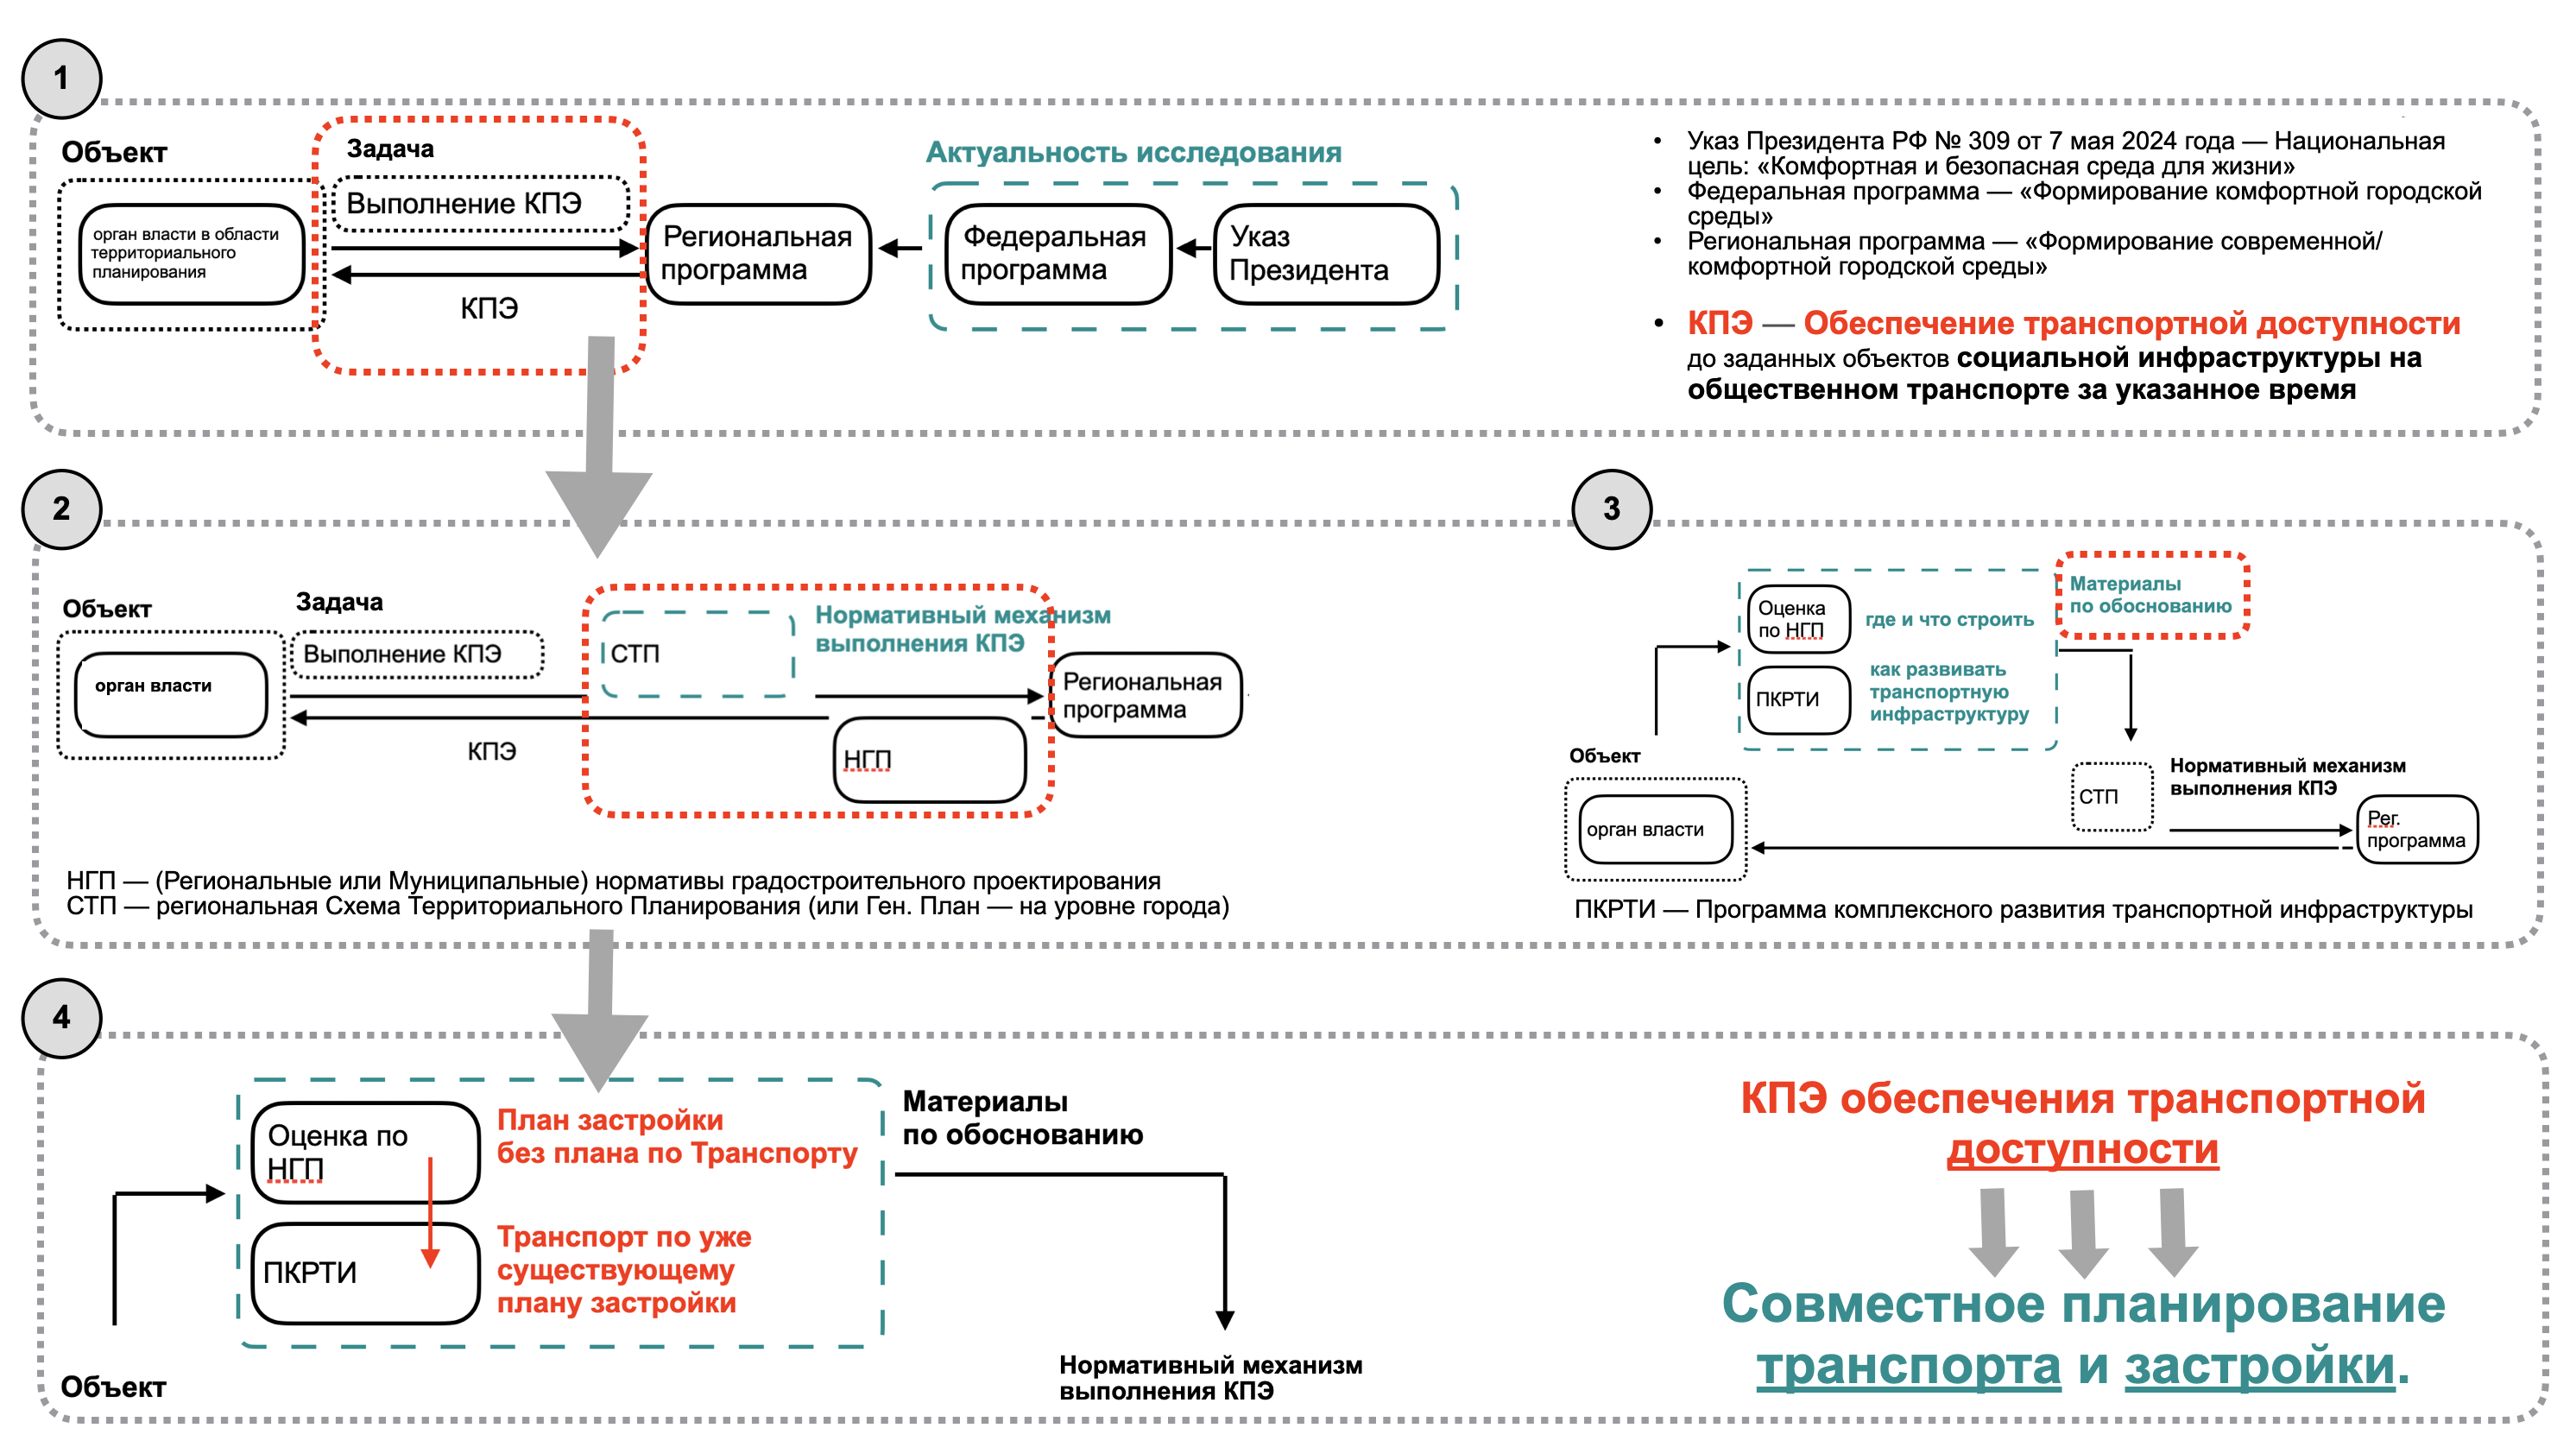
\includegraphics[width=\linewidth]{images/1}
    \caption{Схематичное изображение актуальности проблемы обеспечения транспортной доступности.}
\end{figure}

\begin{figure}[H]
    \centering
    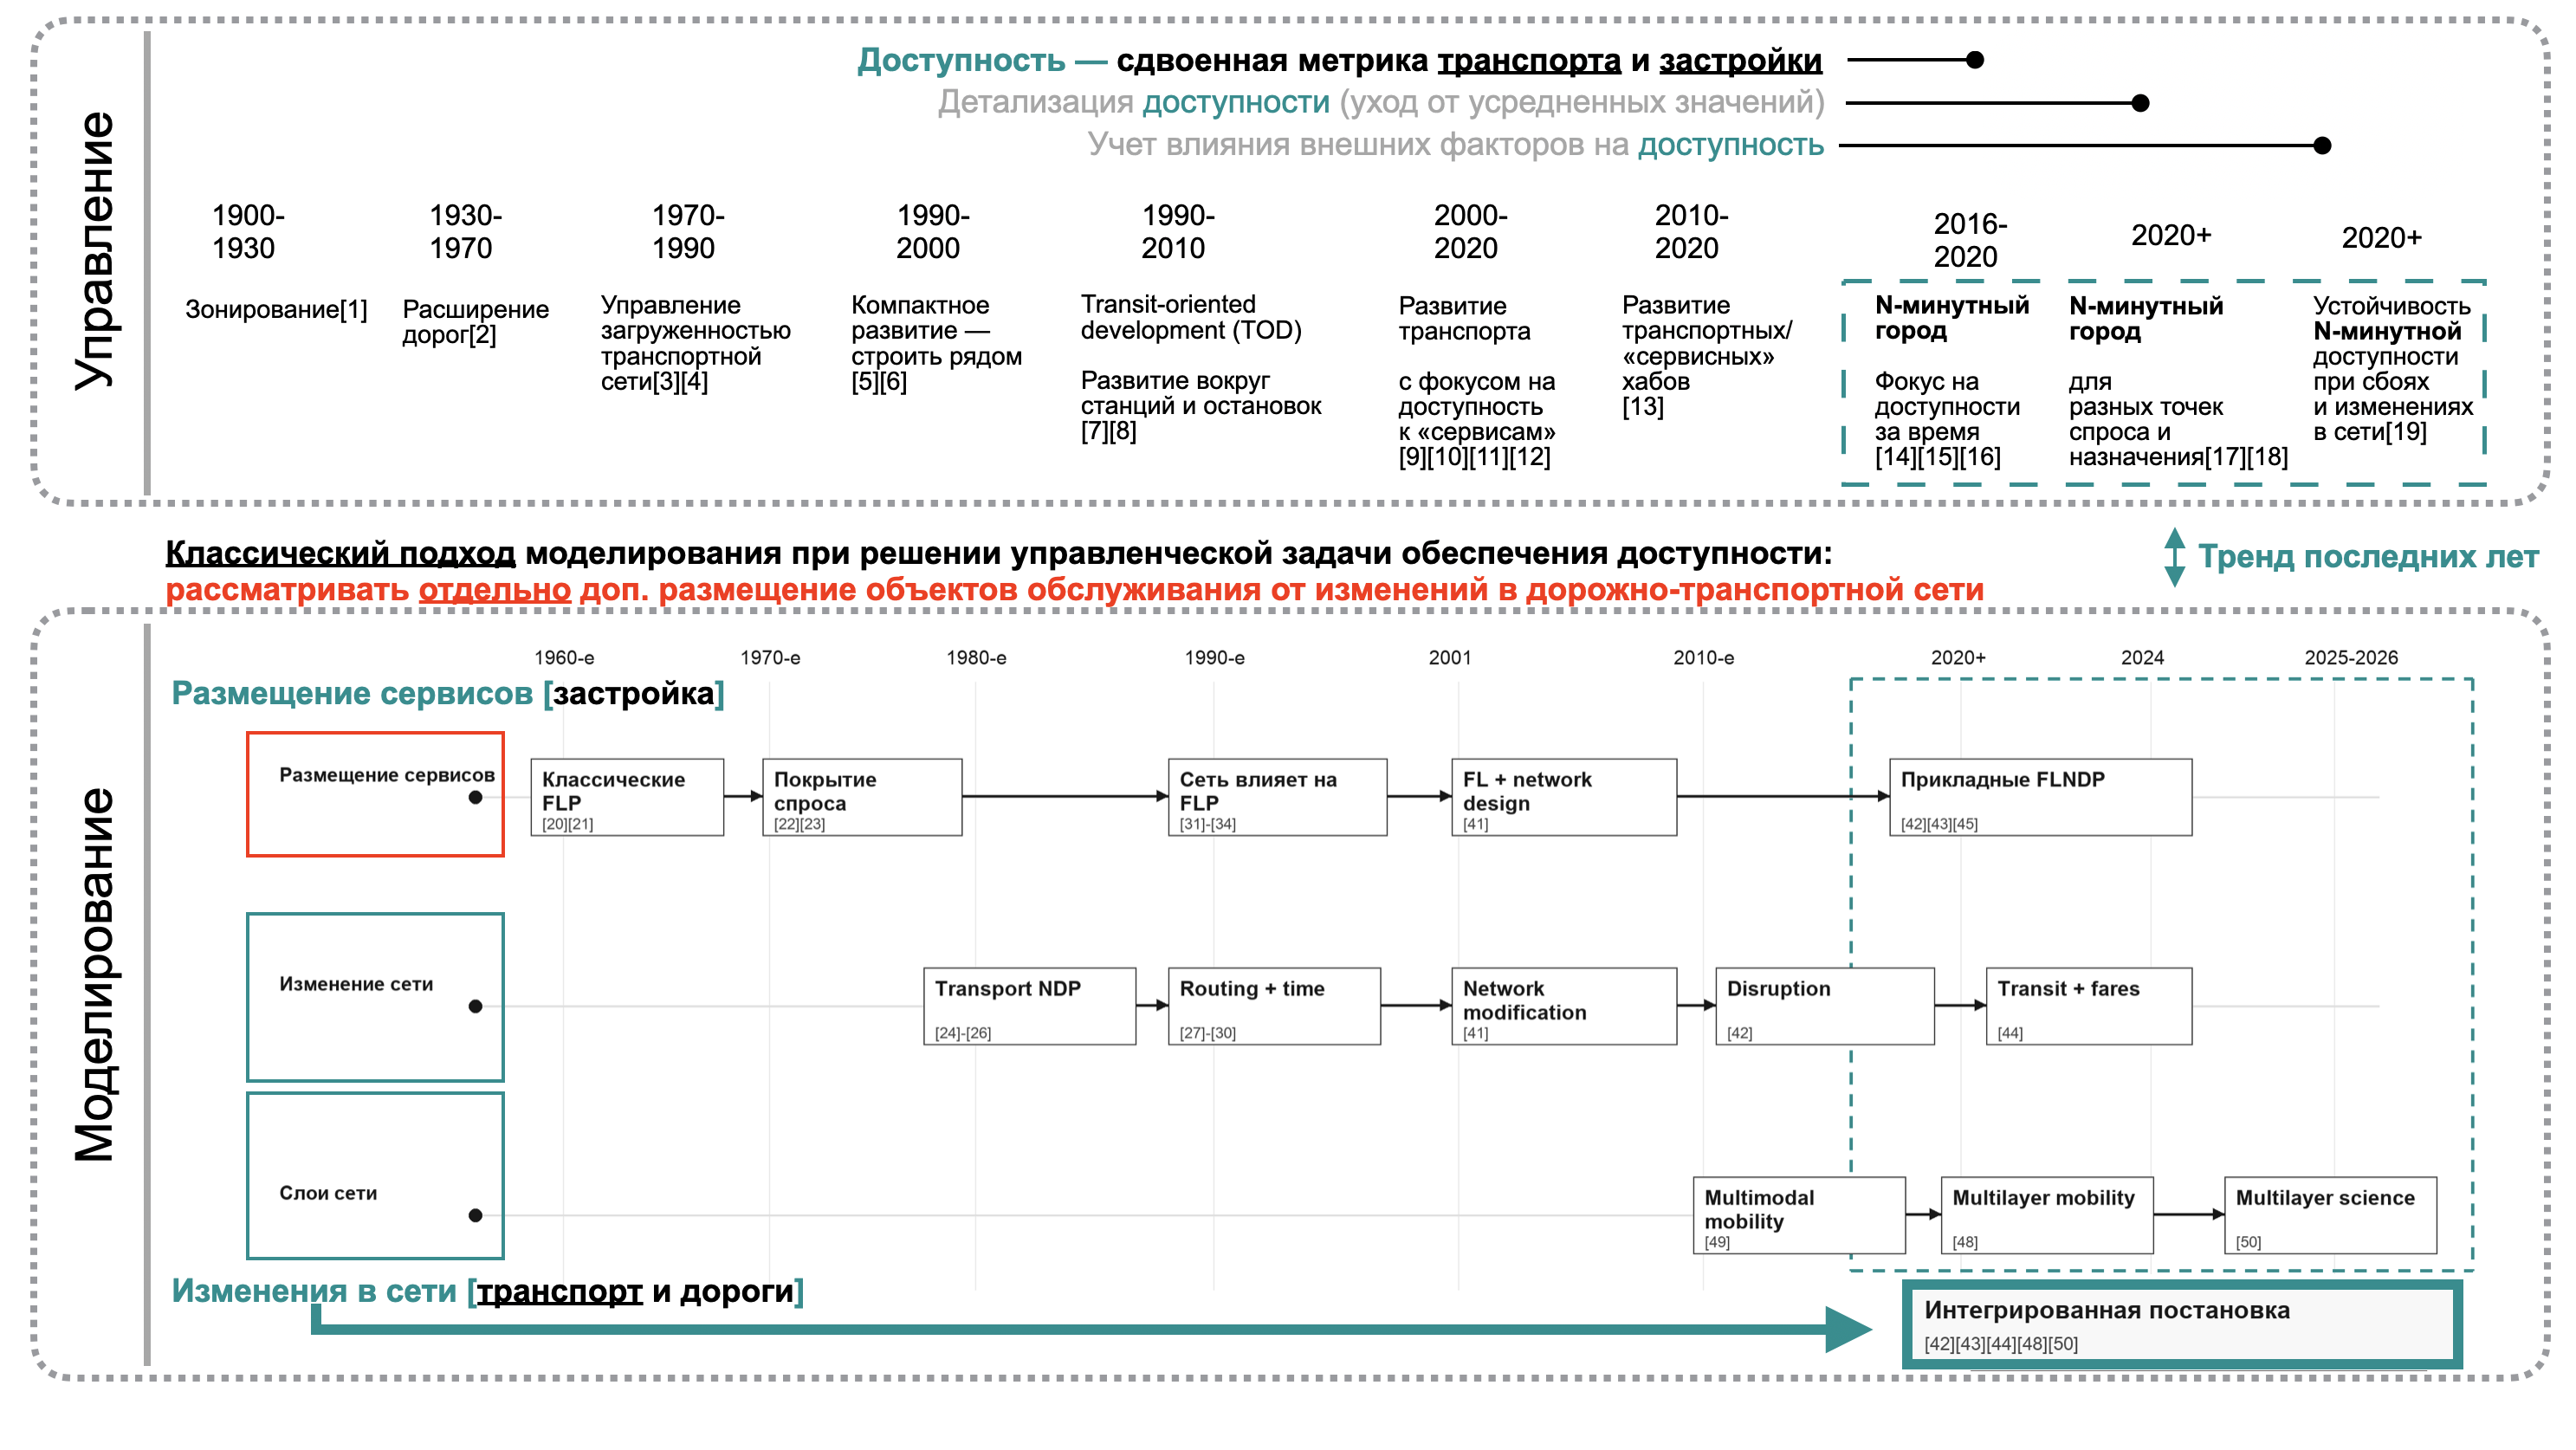
\includegraphics[width=\linewidth]{images/2}
    \caption{Управленческо-методологическая сегментация подходов к решению задачи обеспечения доступности.}
\end{figure}

\begin{figure}[H]
    \centering
    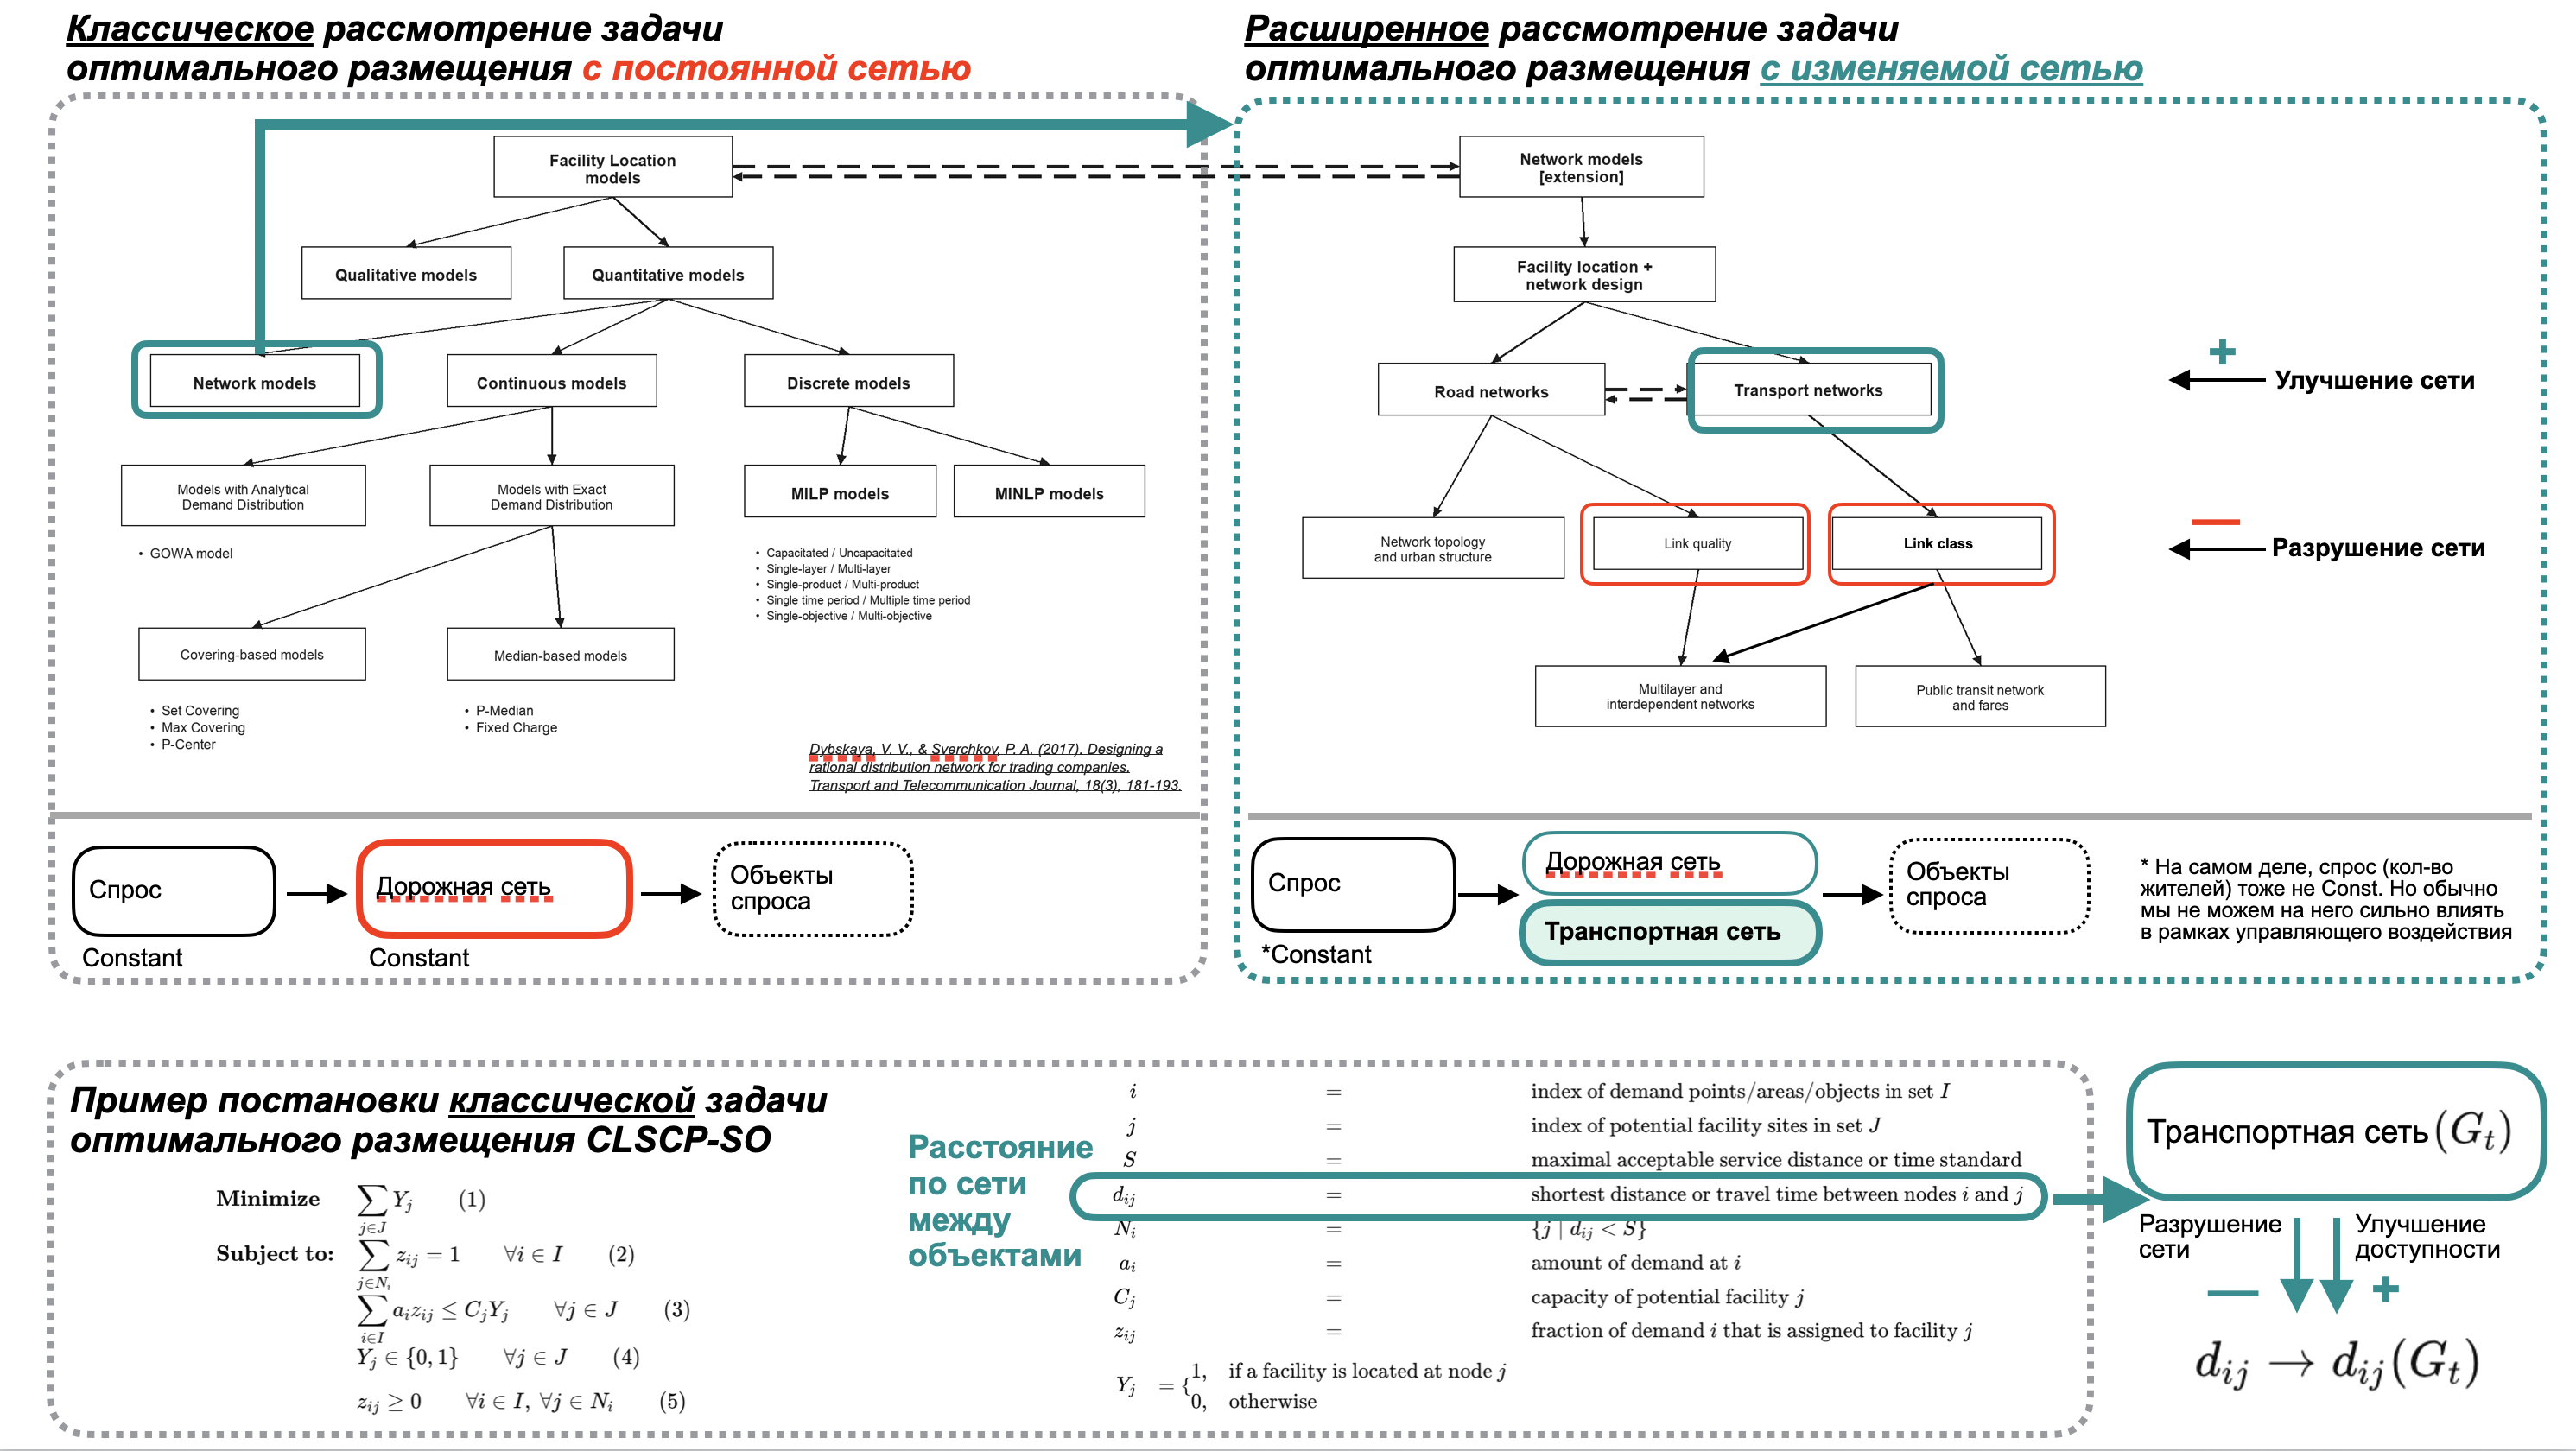
\includegraphics[width=\linewidth]{images/3}
    \caption{Расширение задачи об оптимальном размещении с учетом изменений состояний транспортной сети.}
\end{figure}

\begin{figure}[H]
    \centering
    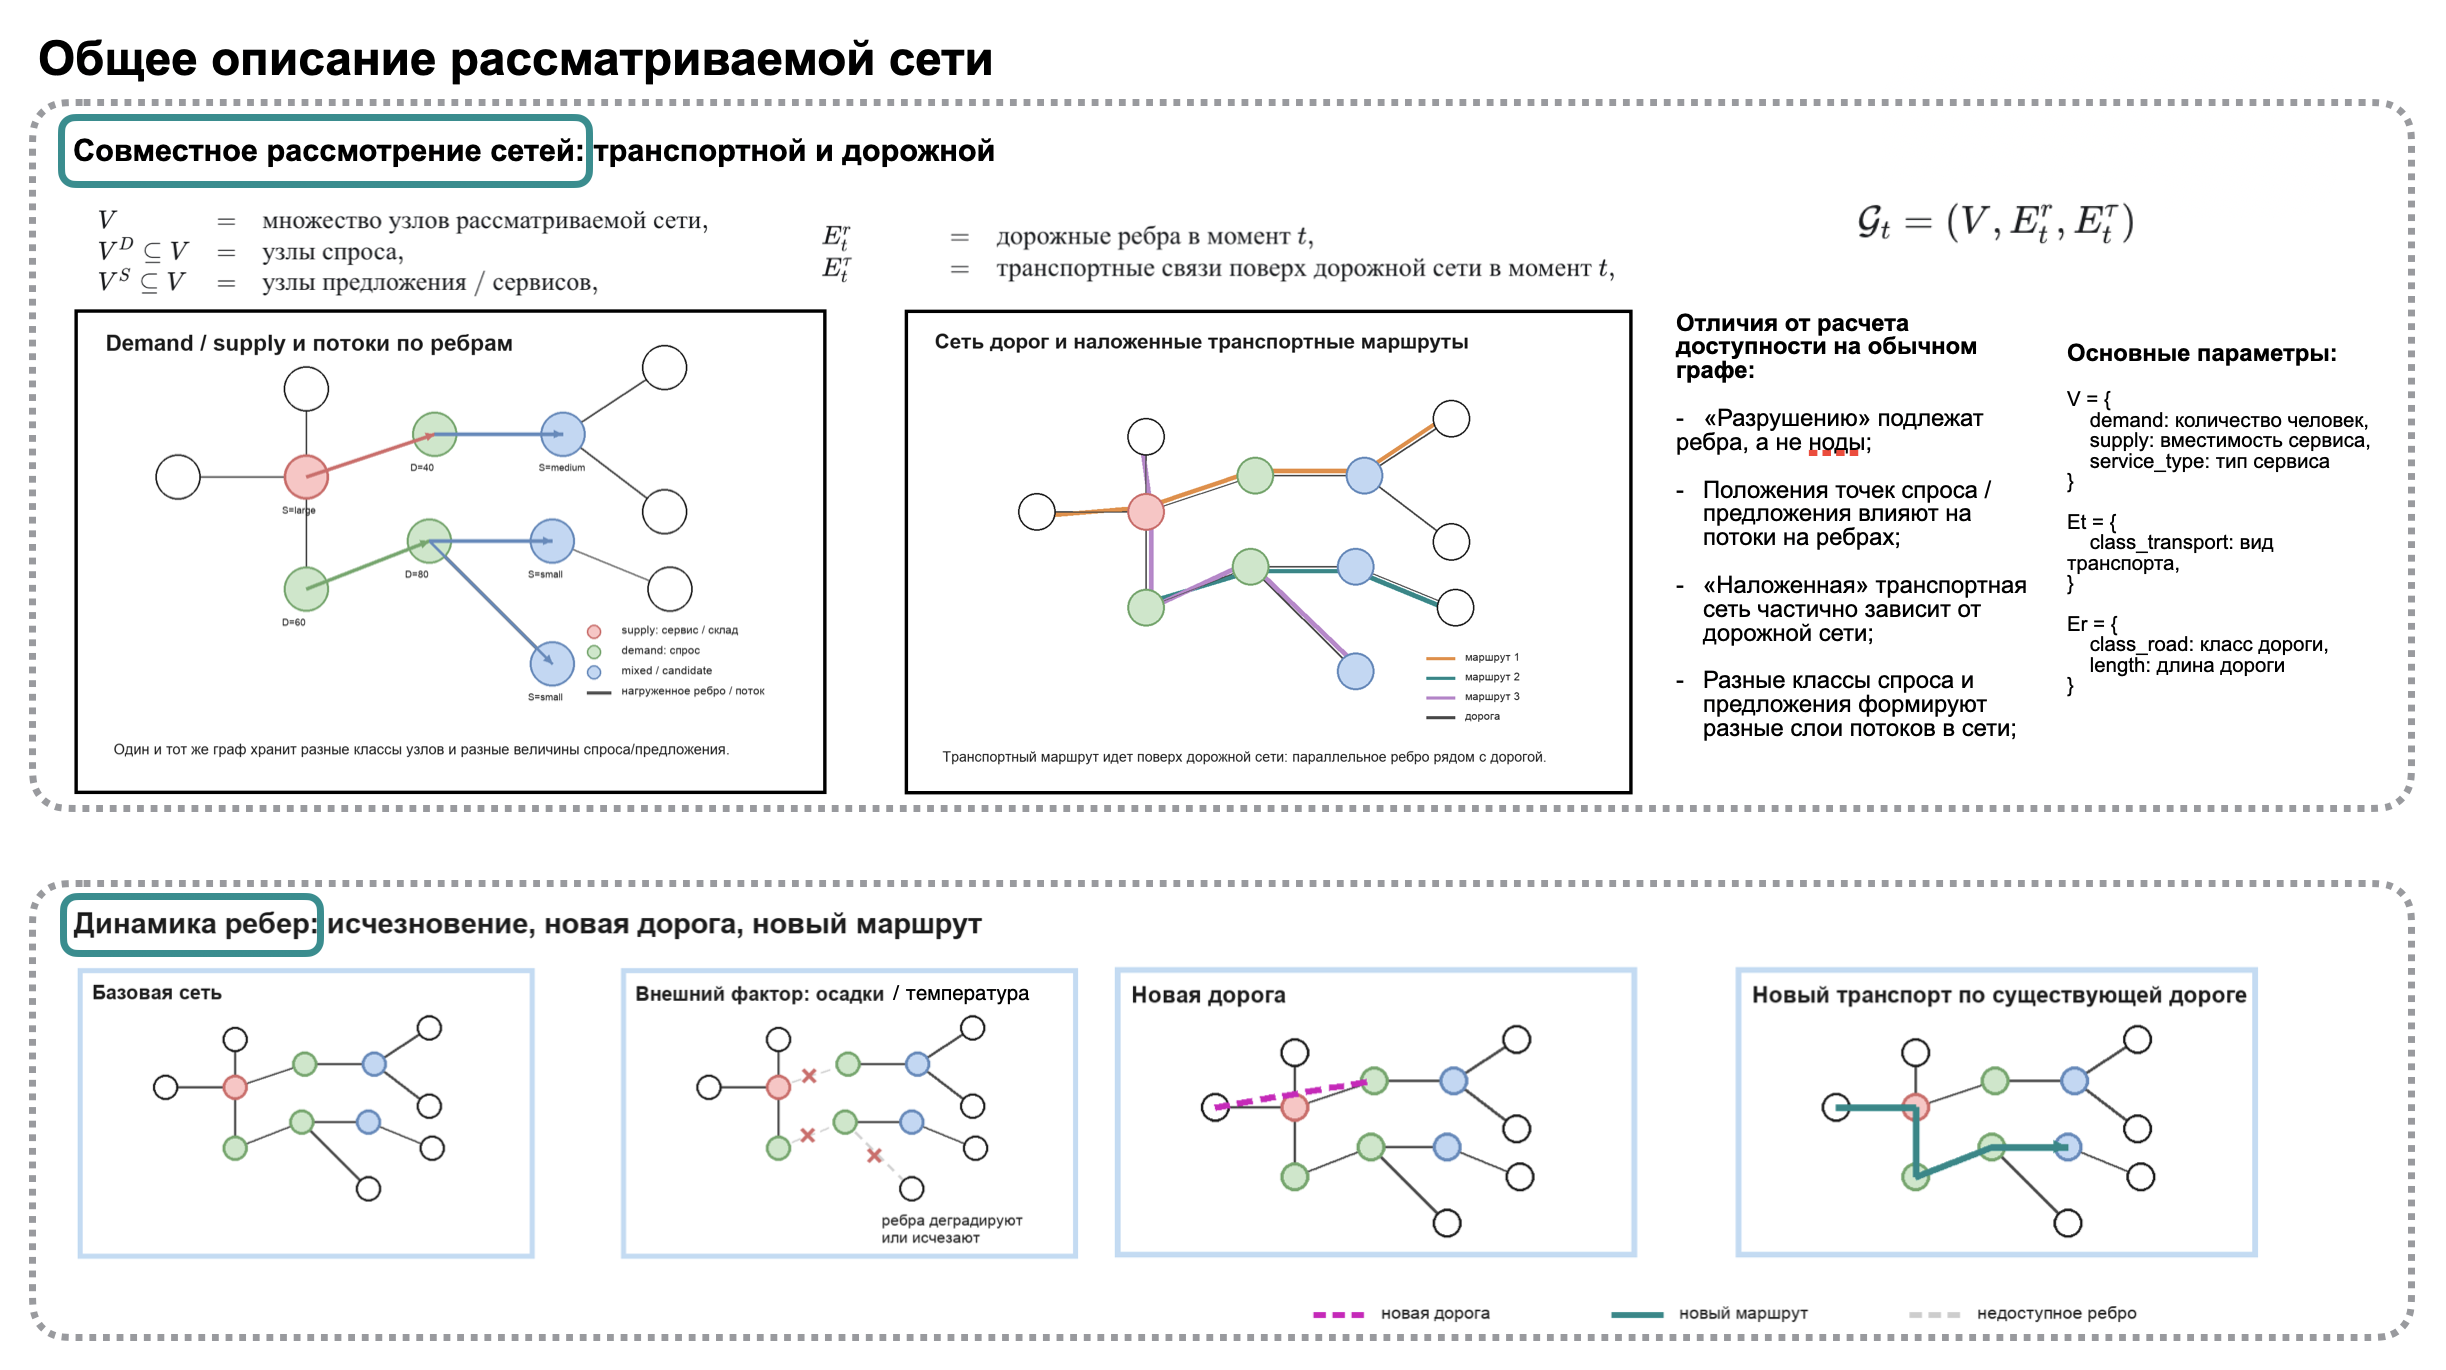
\includegraphics[width=\linewidth]{images/4}
    \caption{Общая схема рассматриваемой сети.}
\end{figure}

\begin{figure}[H]
    \centering
    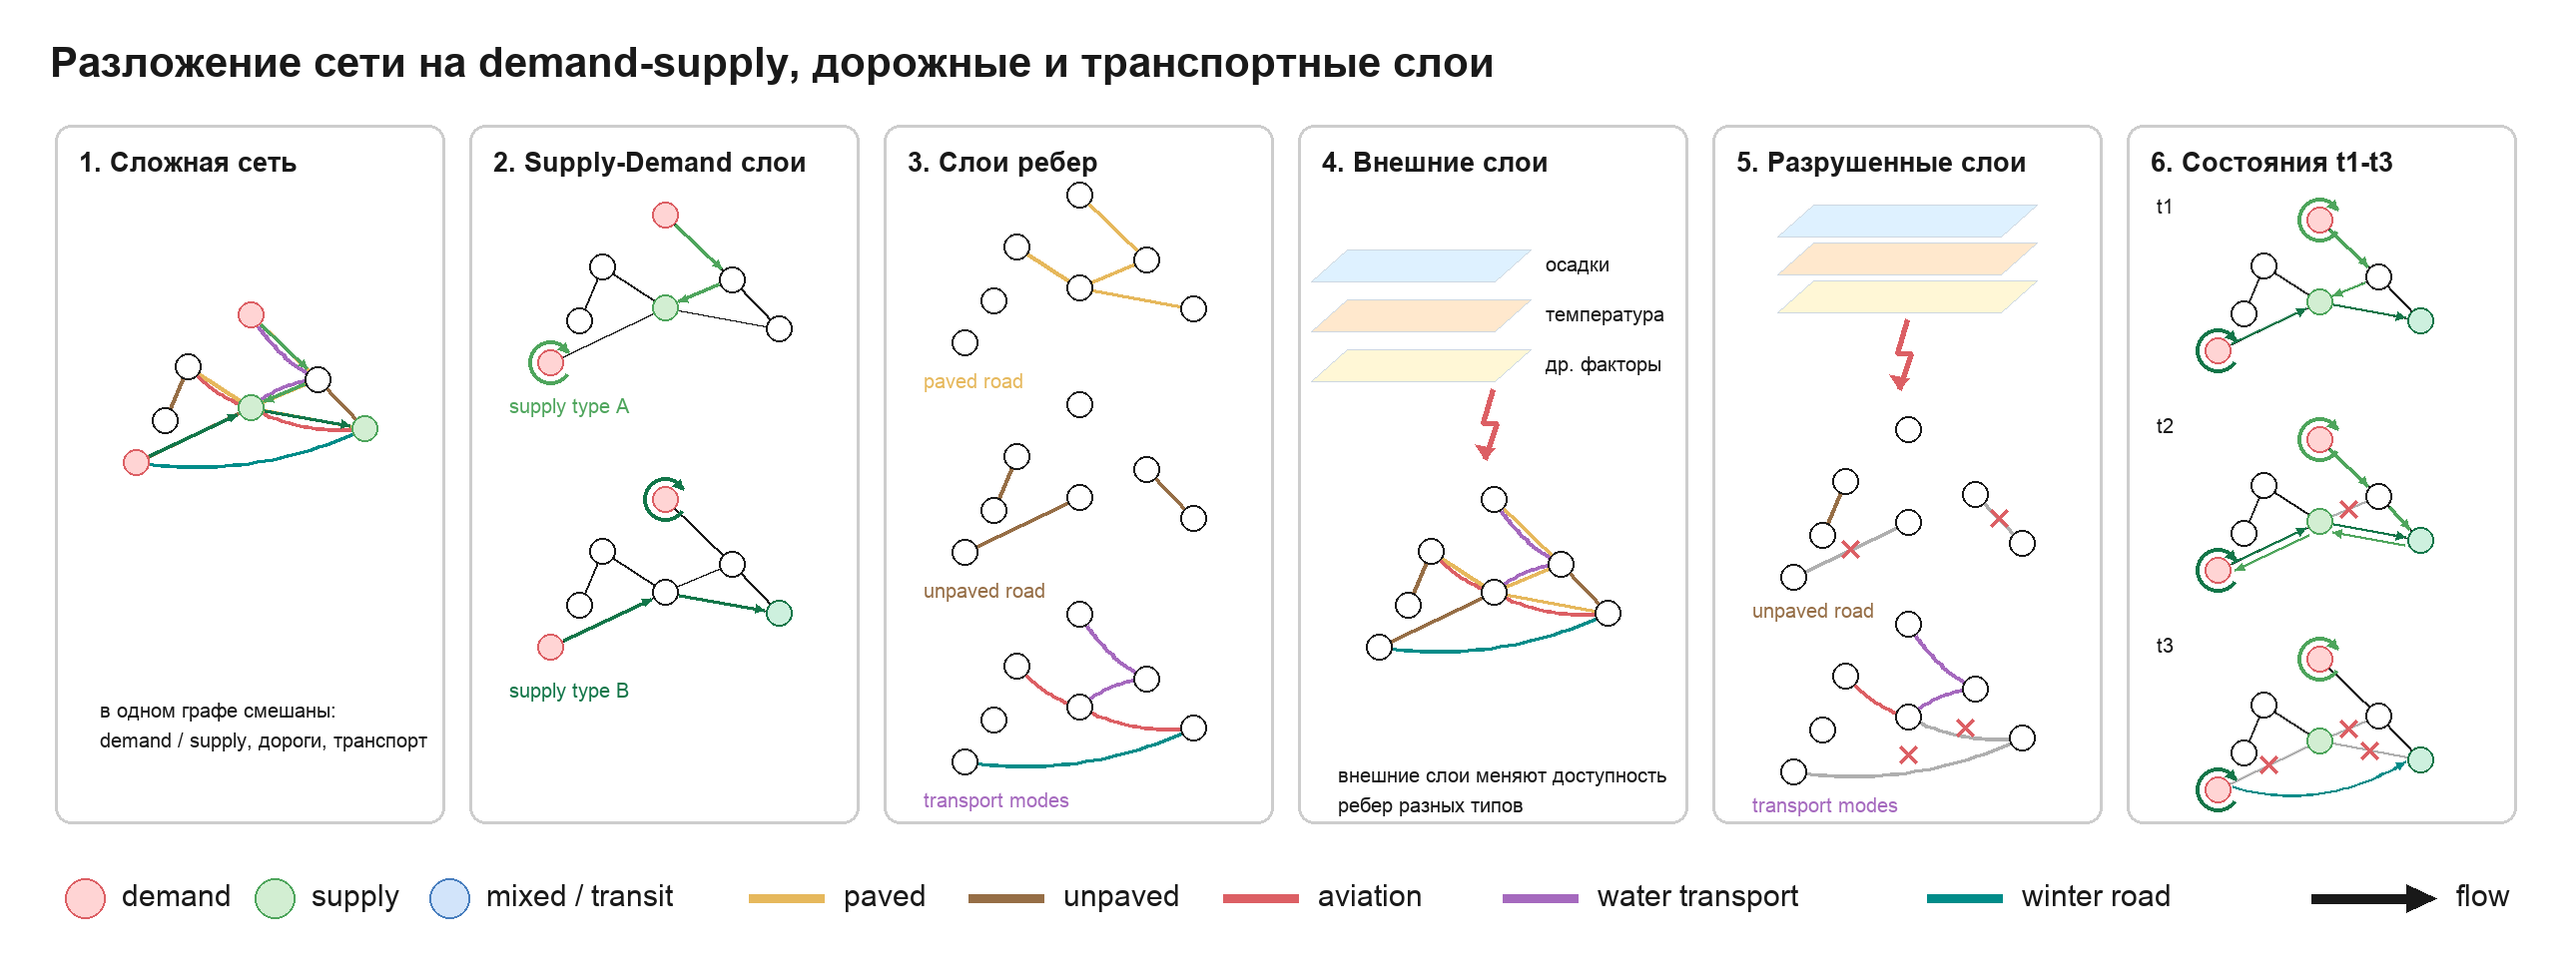
\includegraphics[width=\linewidth]{images/5}
    \caption{Схематичное изображение изменения состояния многоуровневой сети под воздействием внешних факторов}
\end{figure}

\begin{figure}[H]
    \centering
    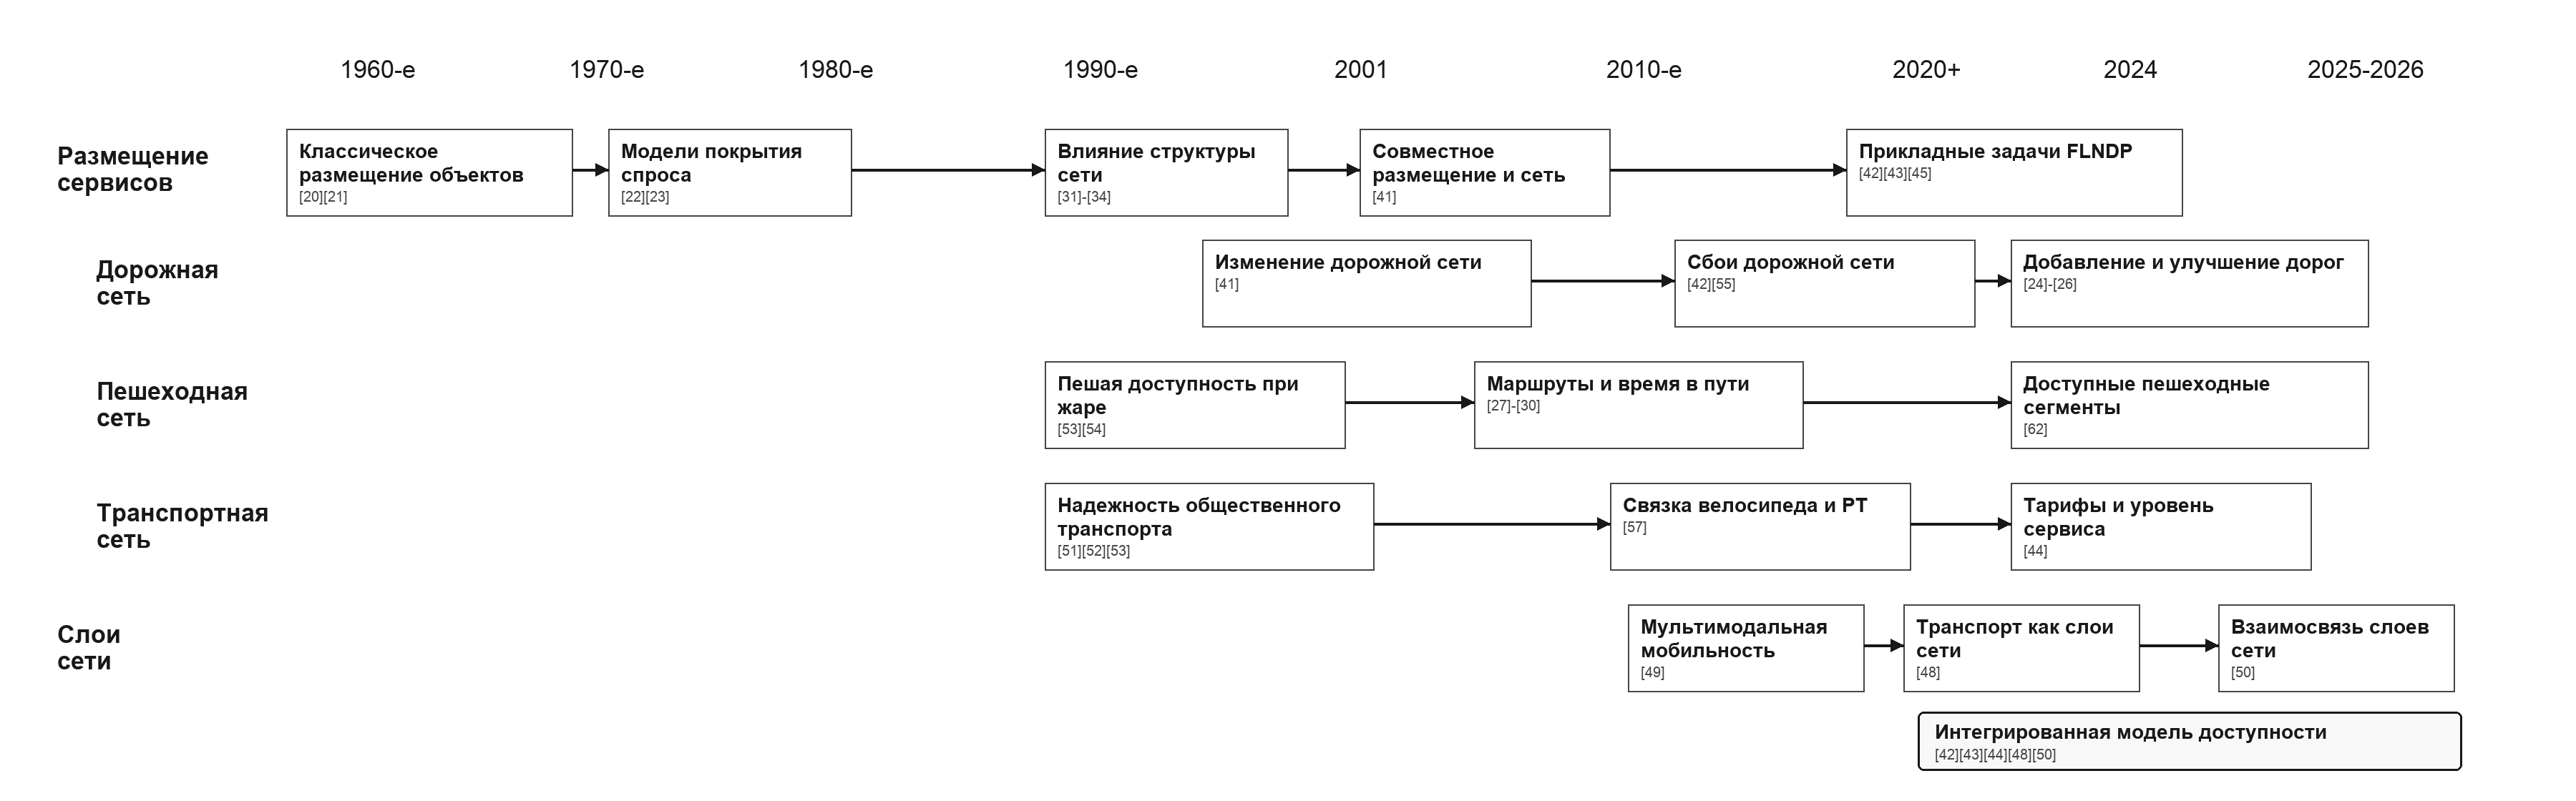
\includegraphics[width=.95\linewidth]{Dissertation/facility_location_tnd_timeline}
    \caption{Таймлайн: facility location + transportation network design}
\end{figure}

\begin{figure}[H]
    \centering
    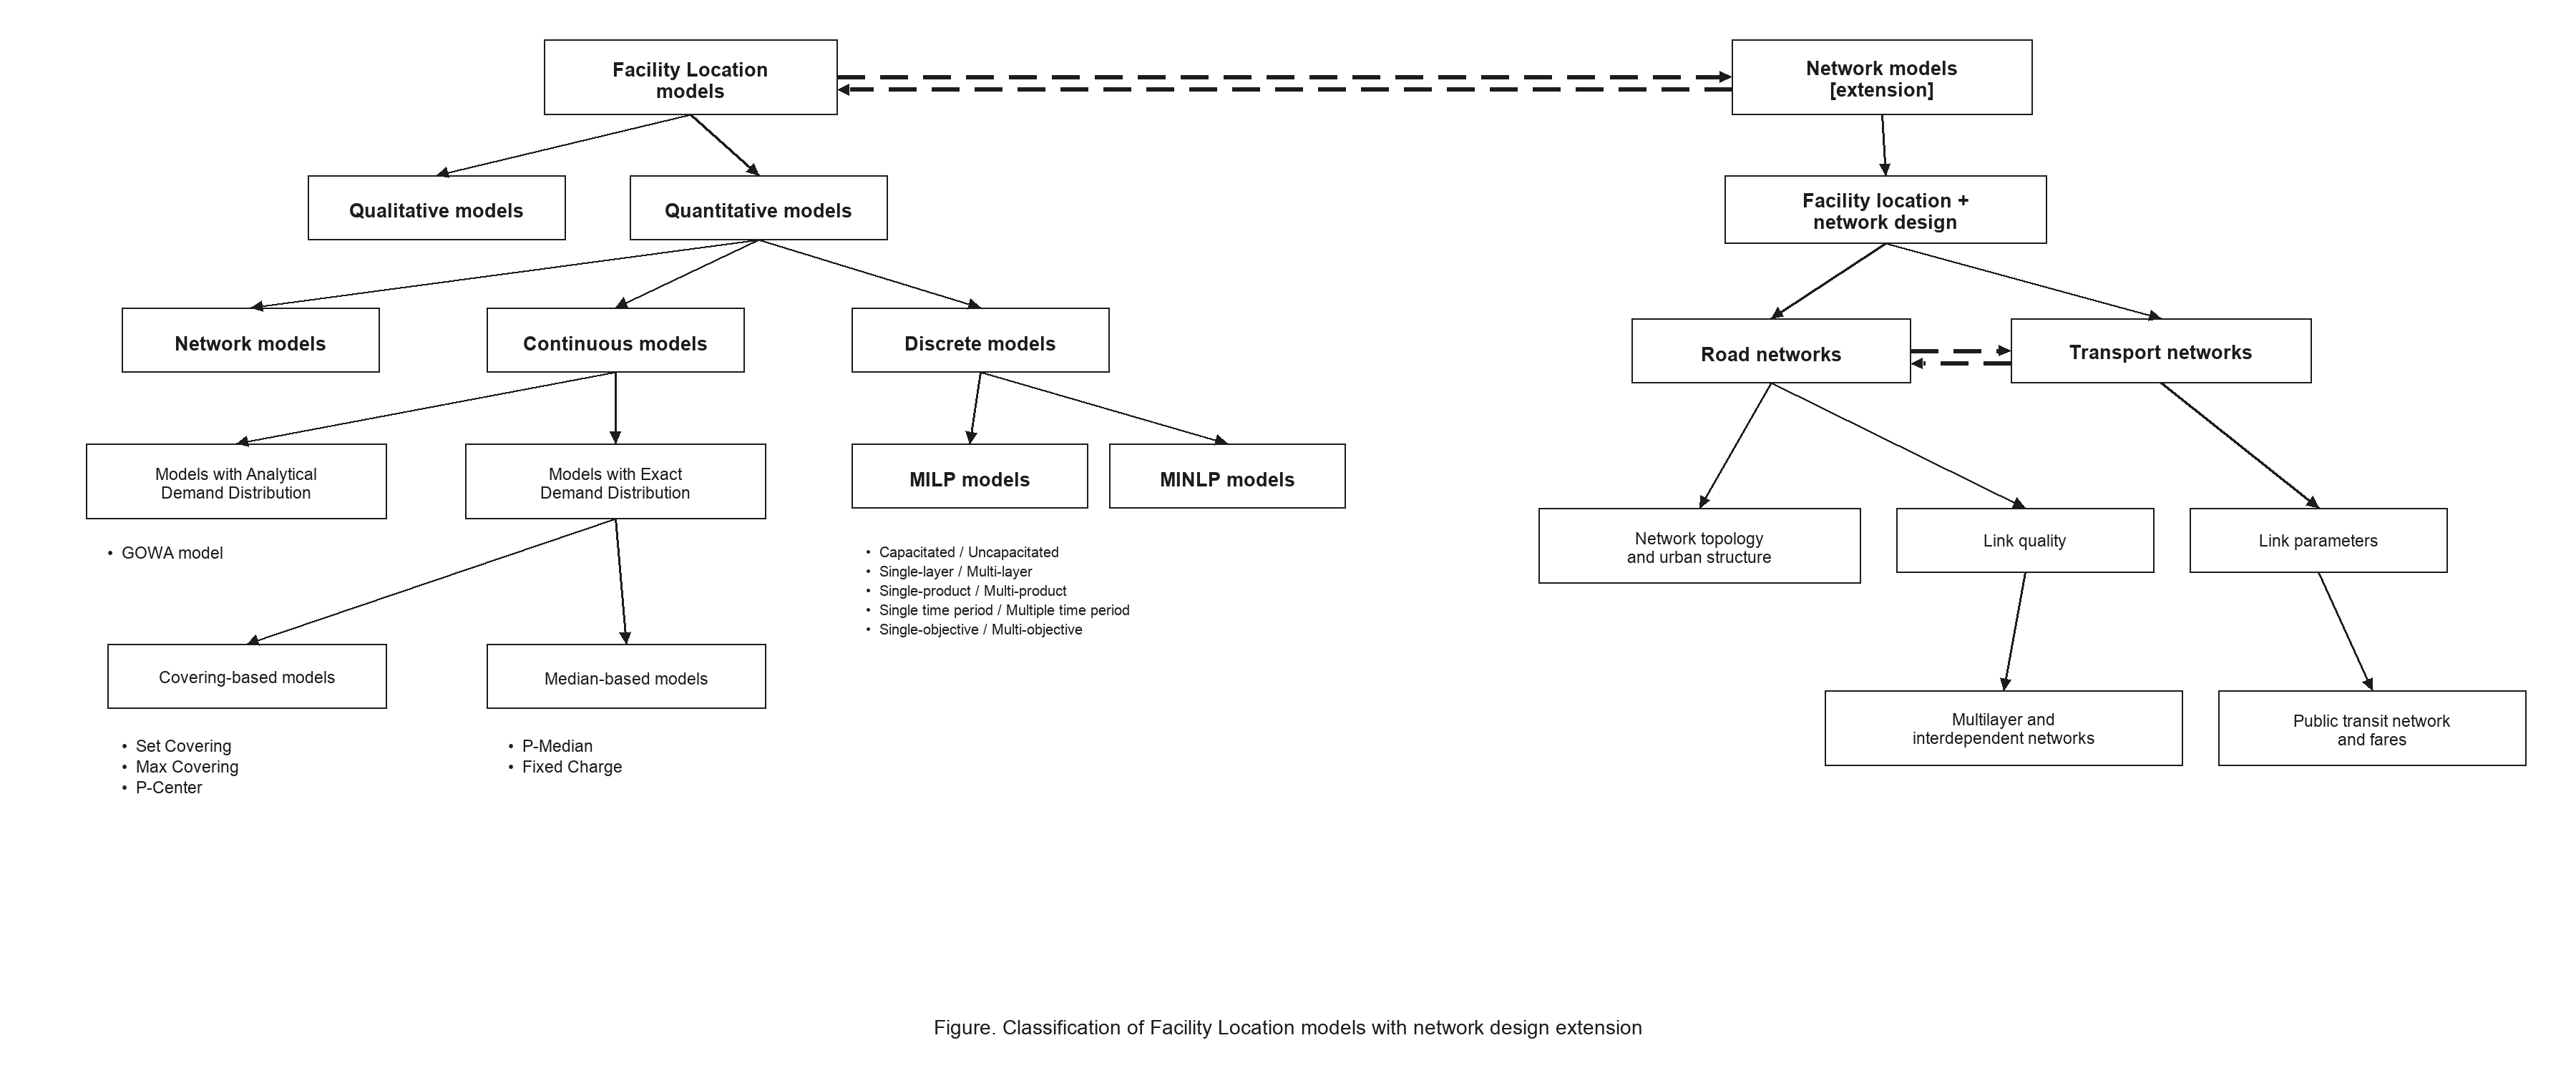
\includegraphics[width=.95\linewidth]{Dissertation/facility_location_network_design_classification}
    \caption{Схема классификации facility location + network design models}
\end{figure}

\begin{figure}[H]
    \centering
    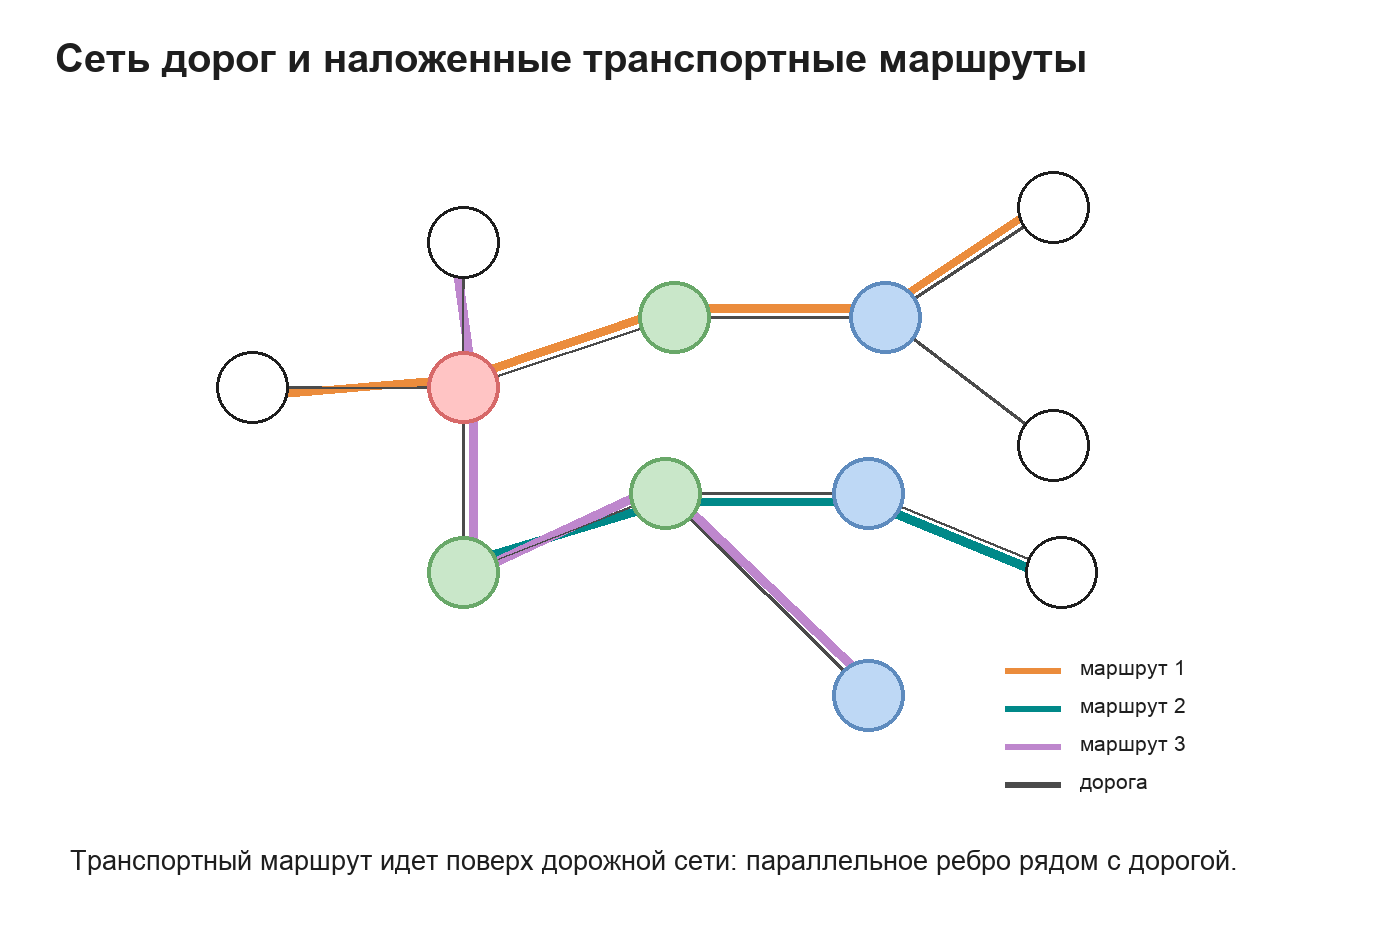
\includegraphics[width=.95\linewidth]{Dissertation/network_routes_schema}
    \caption{Сеть дорог и наложенные транспортные маршруты}
\end{figure}

\begin{figure}[H]
    \centering
    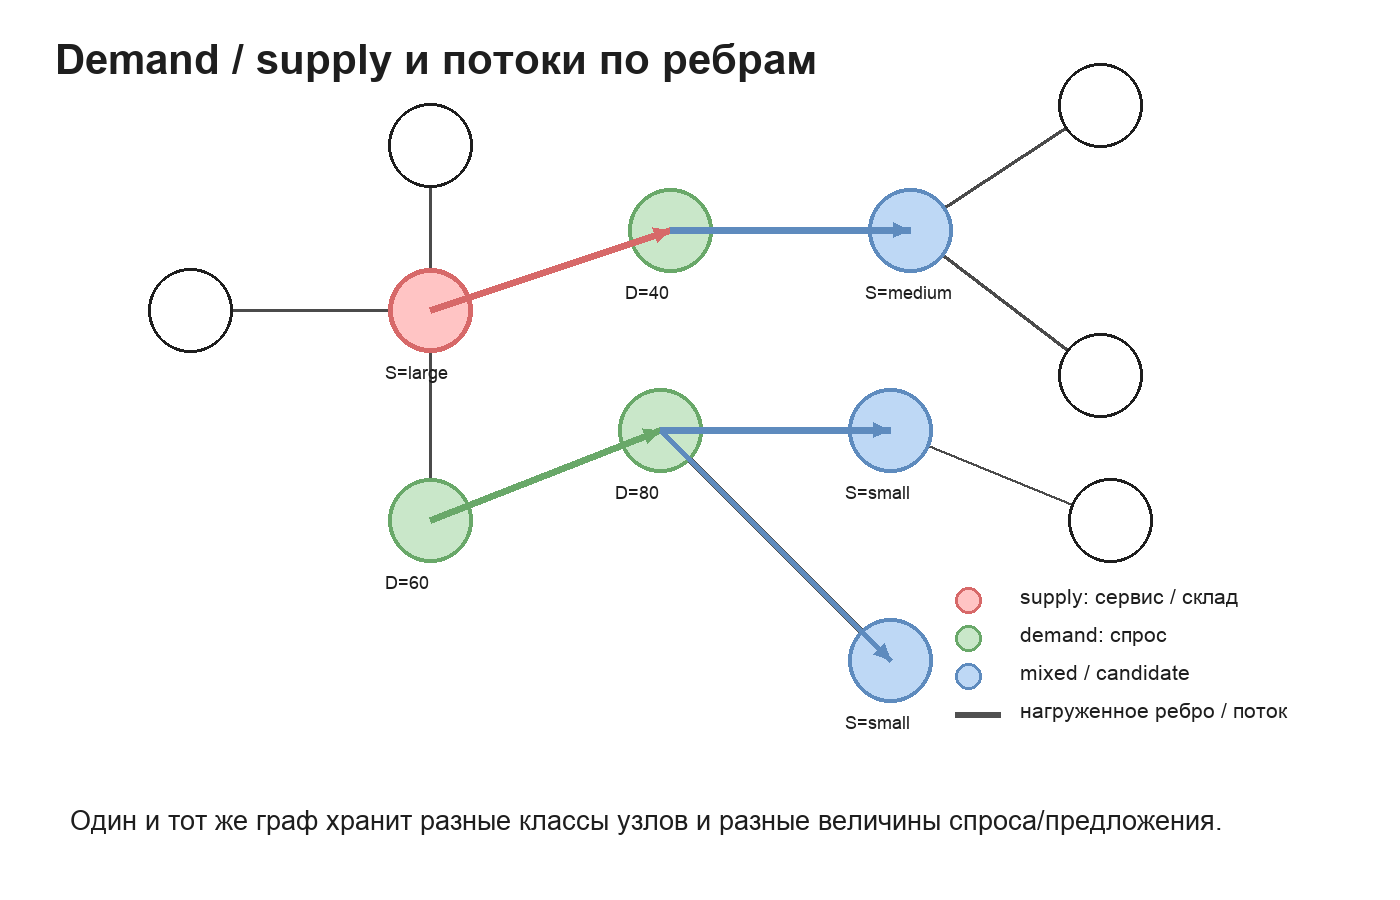
\includegraphics[width=.95\linewidth]{Dissertation/demand_supply_flows_schema}
    \caption{Demand / supply и потоки по ребрам}
\end{figure}

\begin{figure}[H]
    \centering
    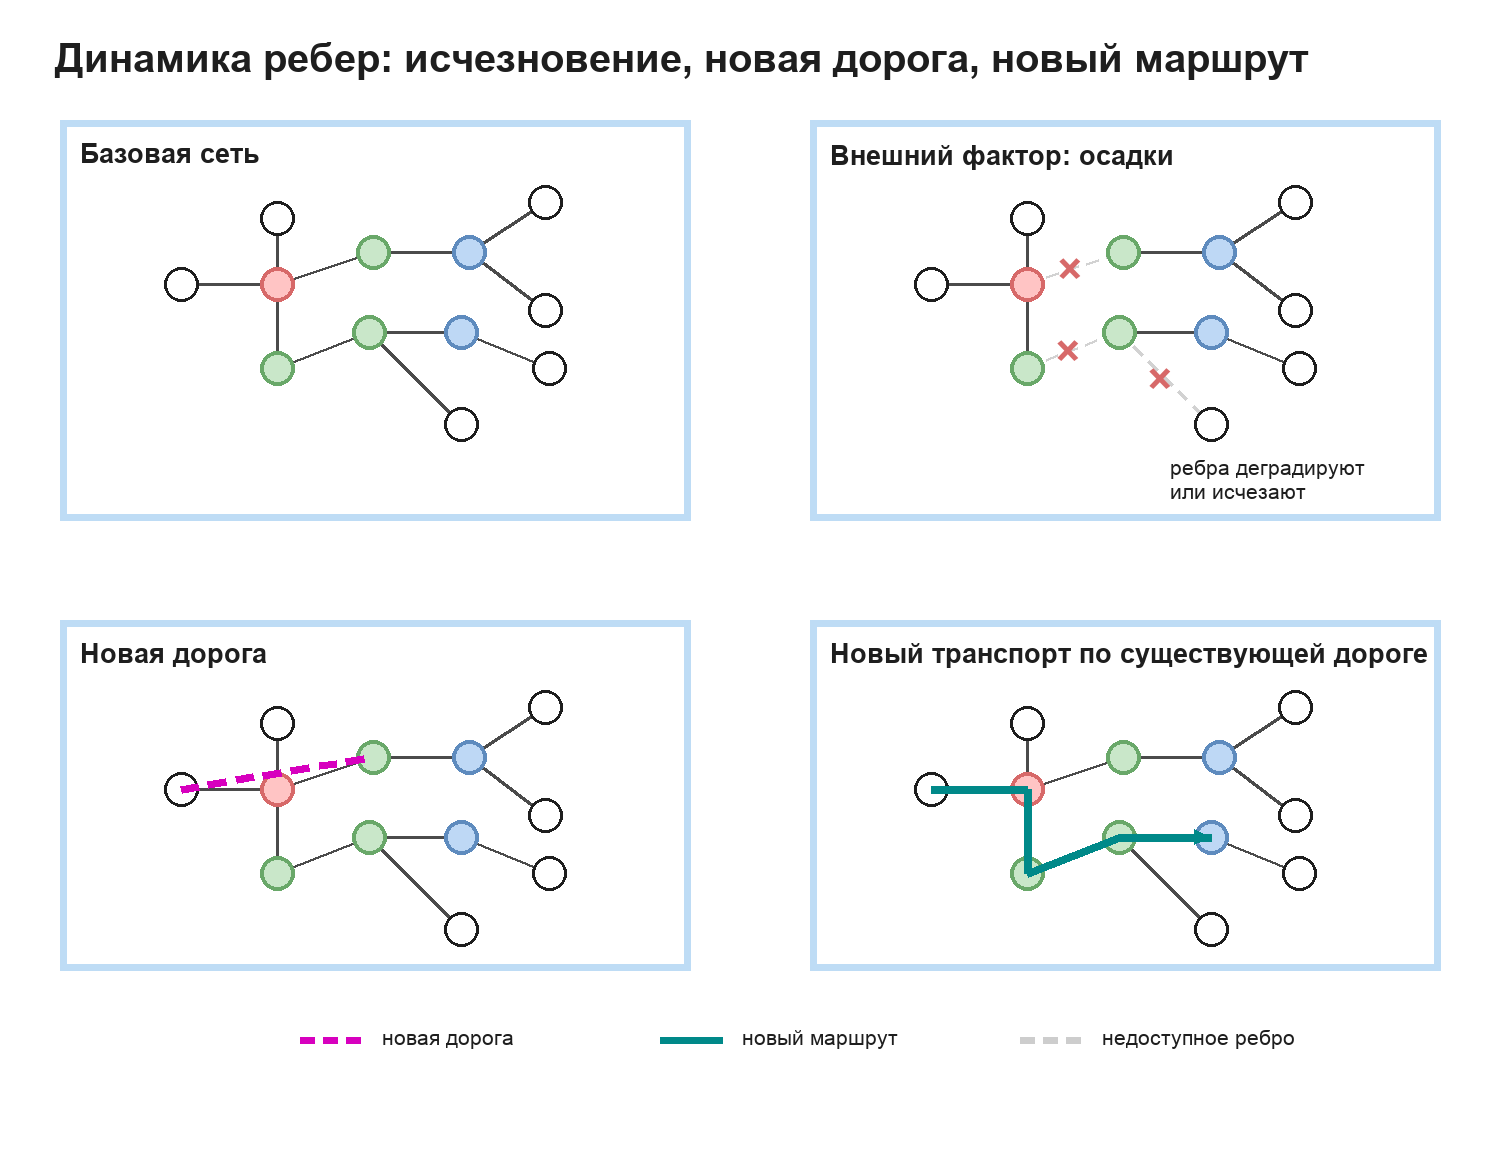
\includegraphics[width=.95\linewidth]{Dissertation/dynamic_edges_schema}
    \caption{Динамика ребер: исчезновение, новая дорога, новый маршрут}
\end{figure}

\begin{figure}[H]
    \centering
    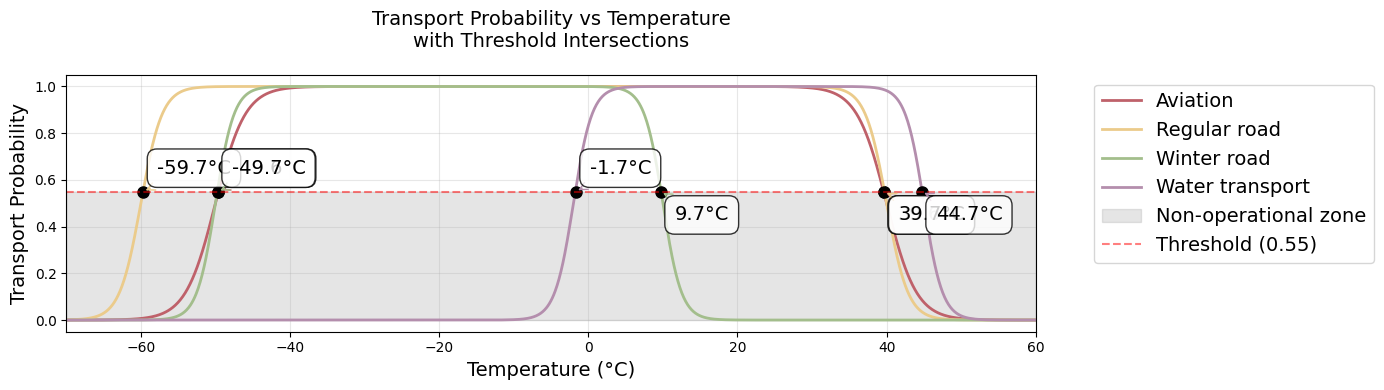
\includegraphics[width=.9\linewidth]{images/ch4/arctic/temp_threshold}
    \caption{Температурно-зависимые условия доступности транспортных режимов в арктическом эксперименте.}
\end{figure}

\begin{figure}[H]
    \centering
    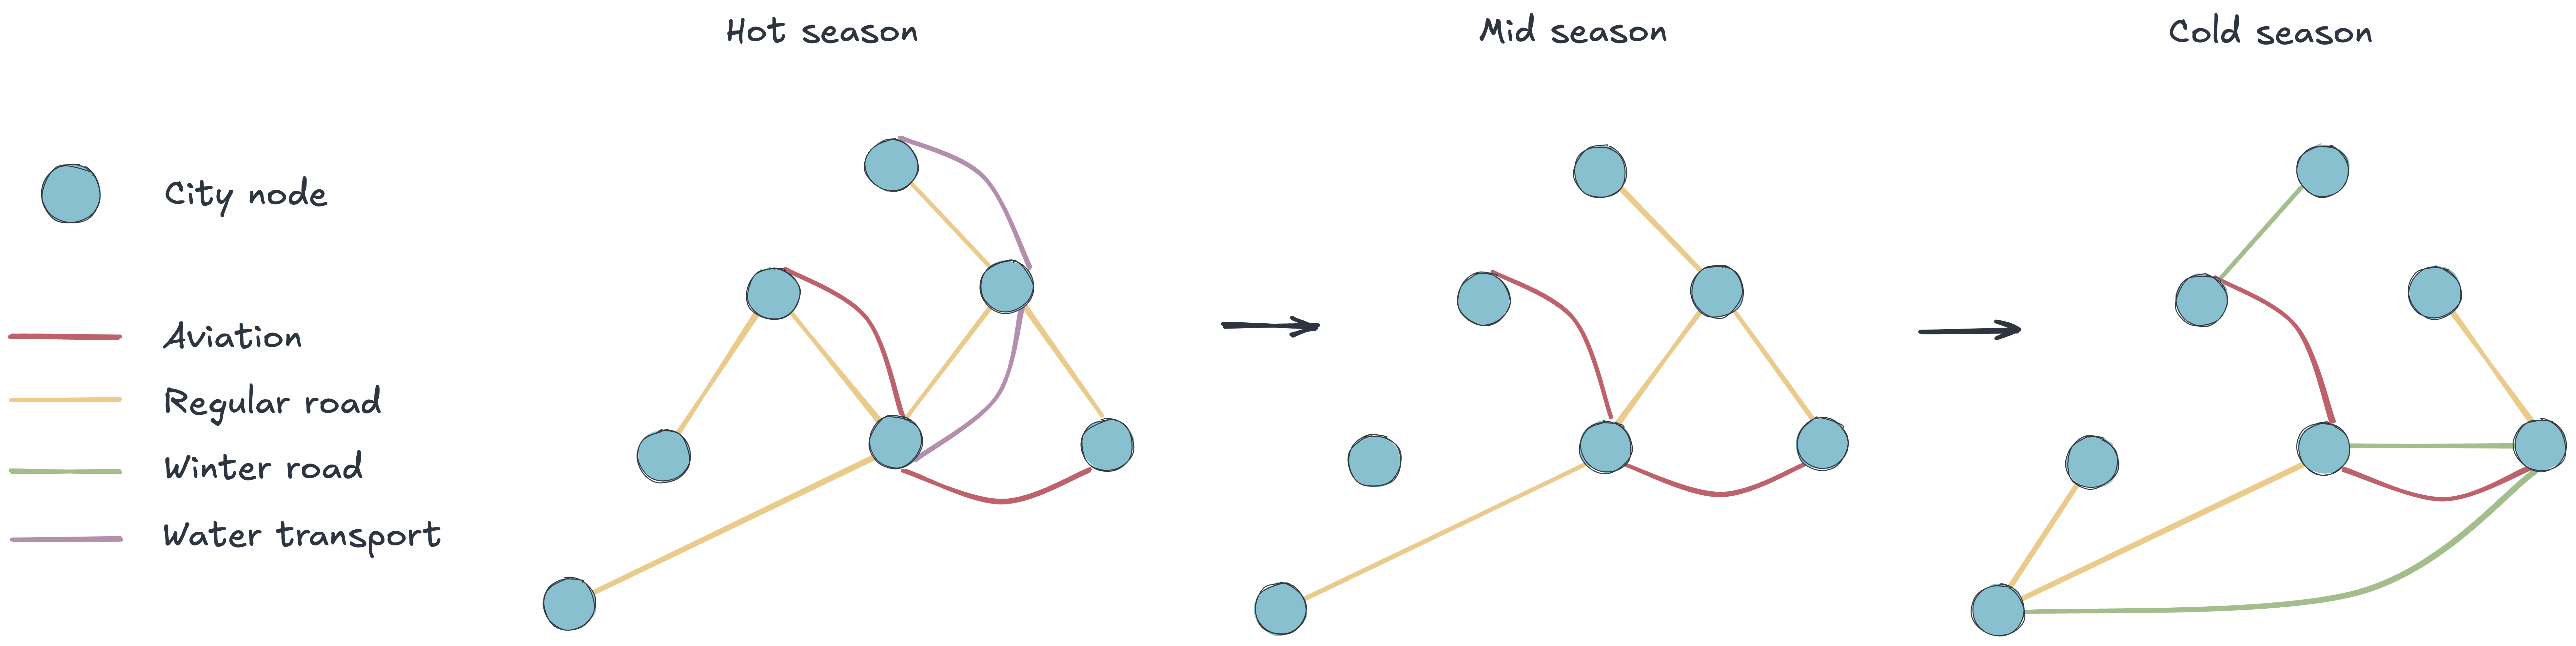
\includegraphics[width=.8\linewidth]{images/ch4/arctic/seasonal_network_scheme}
\end{figure}

\begin{figure}[H]
    \centering
    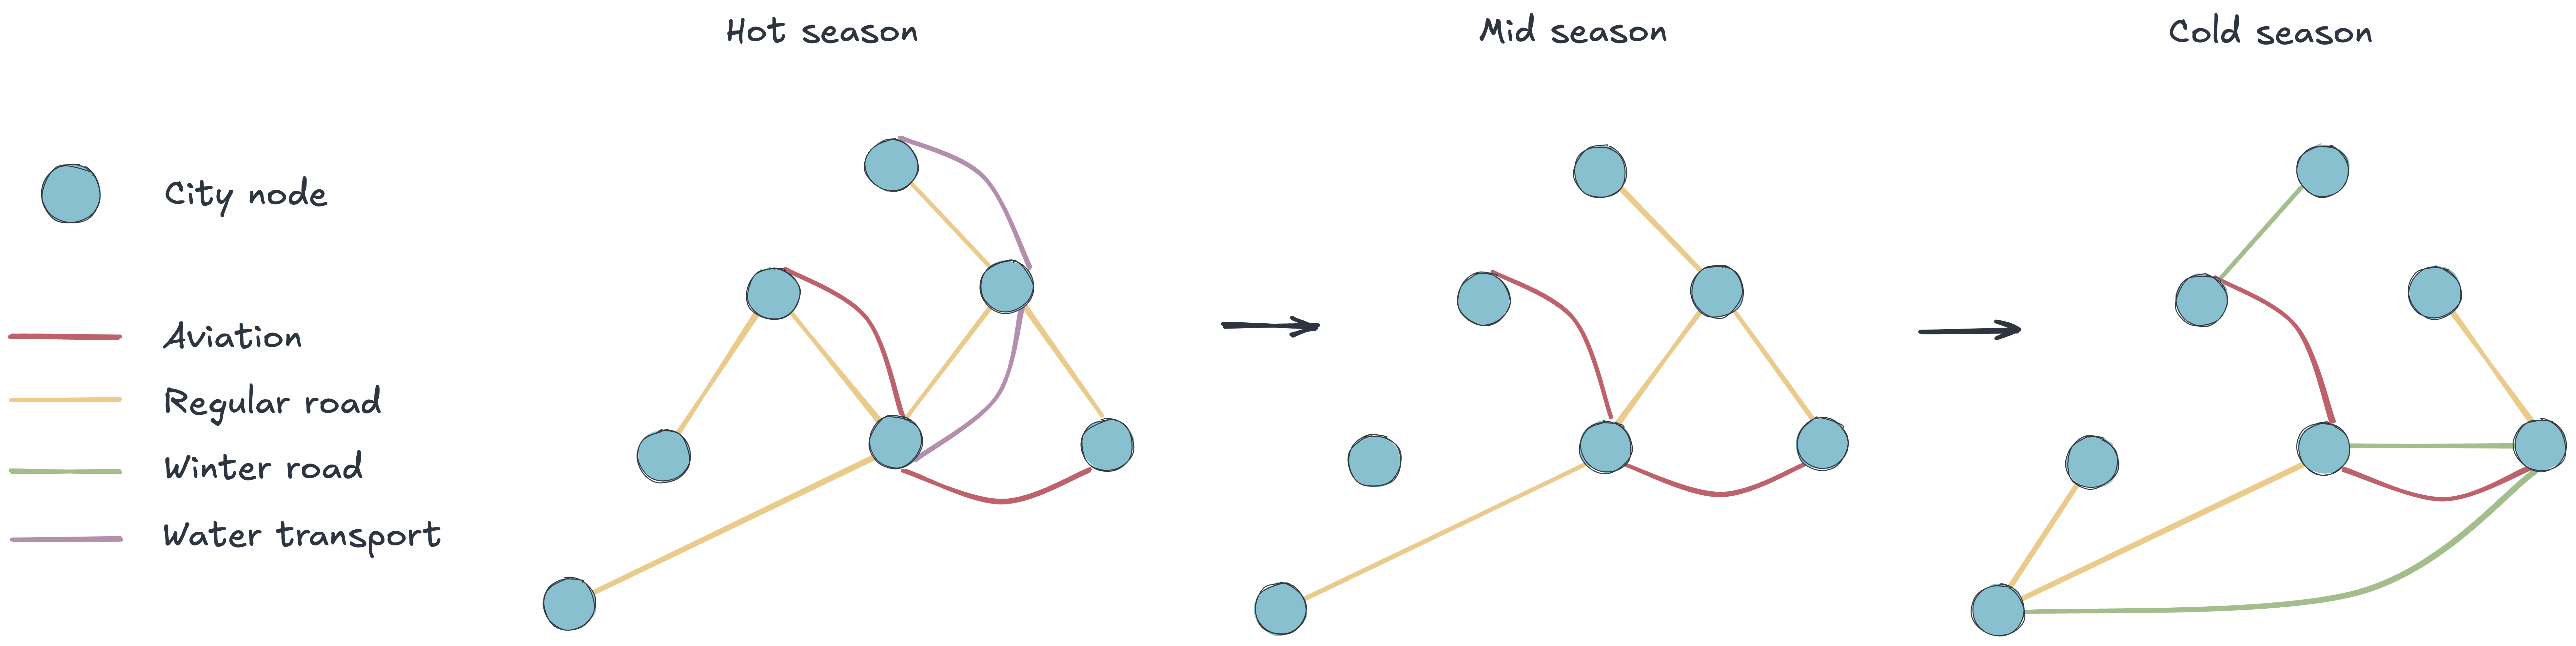
\includegraphics[width=.48\linewidth]{images/ch4/arctic/seasonal_network_scheme_transition}
    \hfill
    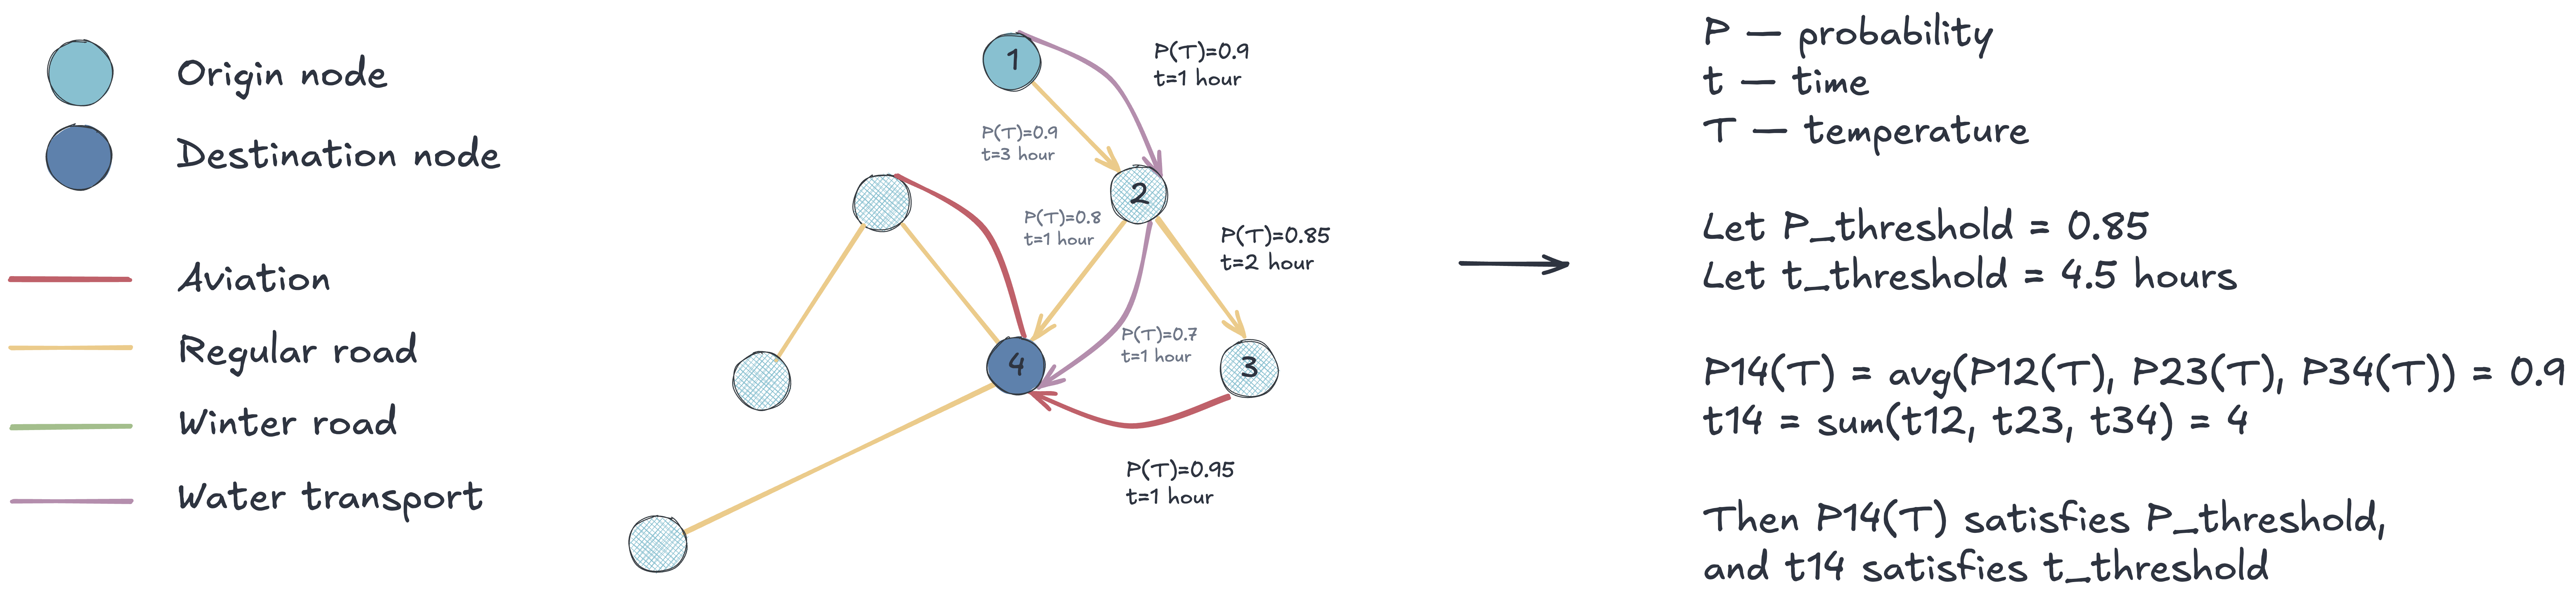
\includegraphics[width=.48\linewidth]{images/ch4/arctic/seasonal_network_scheme_cold}
    \caption{Схема перераспределения потоков между сервисными слоями для переходного и холодного сезонов.}
\end{figure}

\begin{figure}[H]
    \centering
    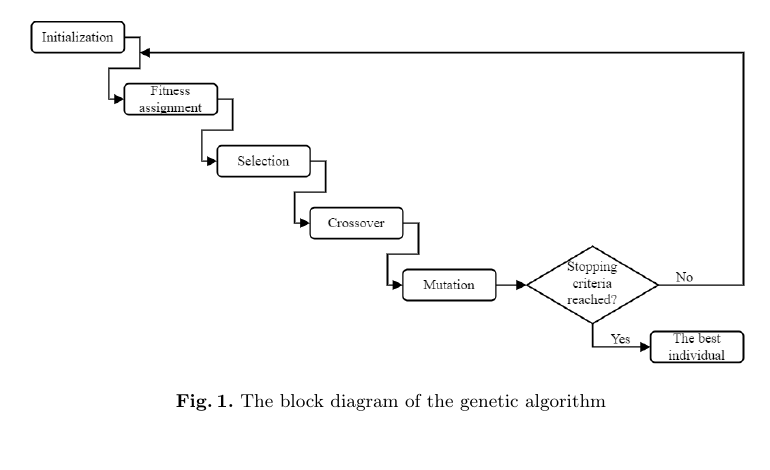
\includegraphics[width=.75\linewidth]{images/tikhevich_toy/tikhevich_ga_block_diagram}
\end{figure}

\begin{figure}[H]
    \centering
    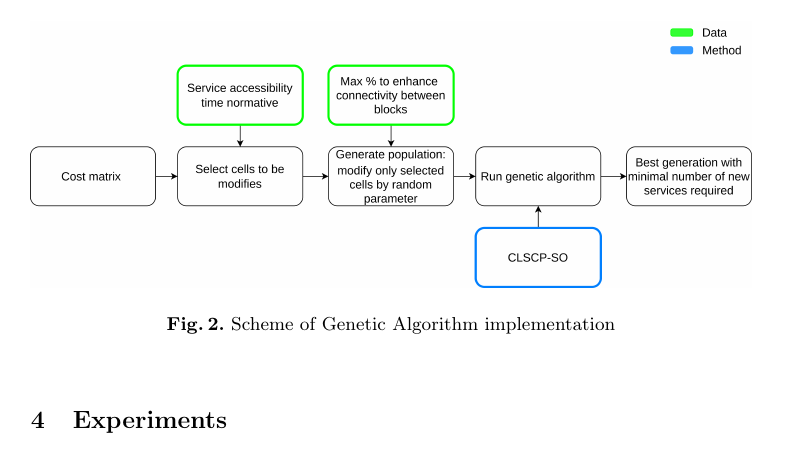
\includegraphics[width=.75\linewidth]{images/tikhevich_toy/tikhevich_ga_implementation_scheme}
    \caption{Схема реализации генетического алгоритма из \cite{kontsevik2024connectivityPlacement}}
\end{figure}

\clearpage
\section*{Результаты}

\begin{figure}[H]
    \centering
    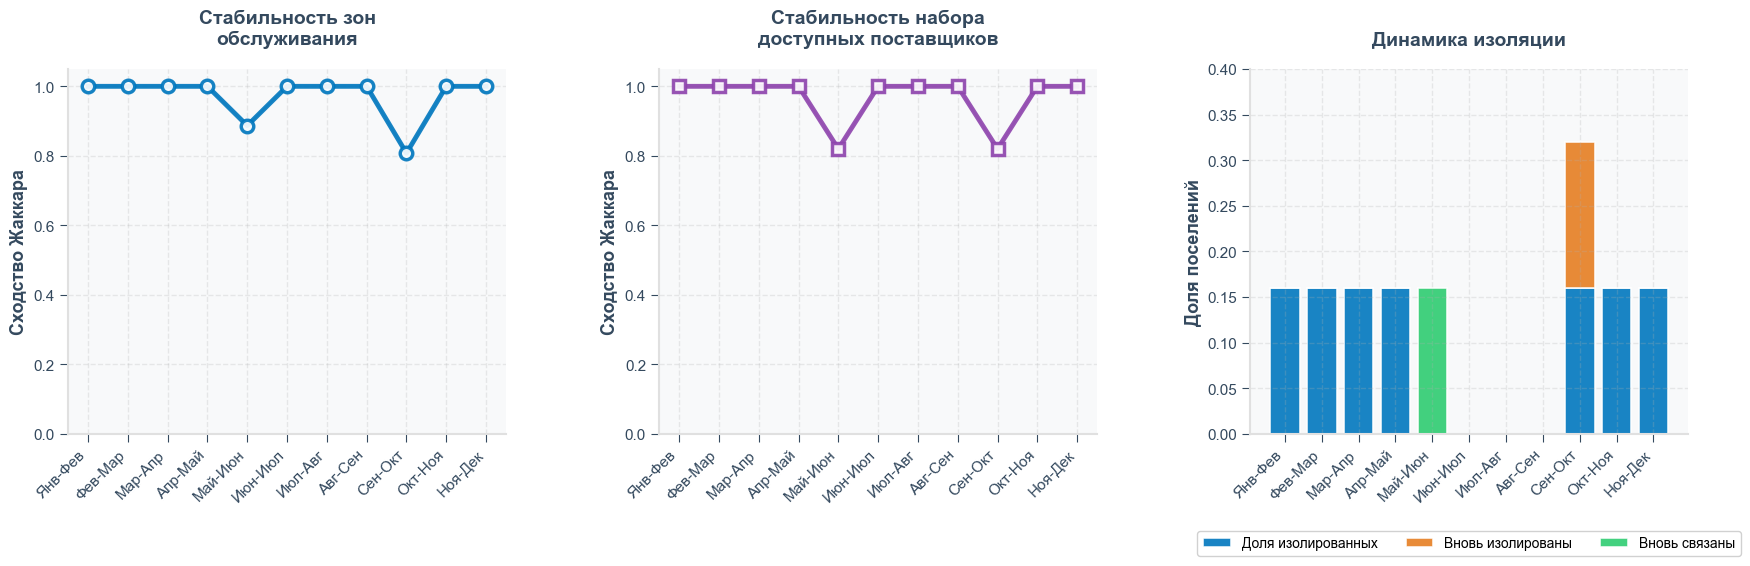
\includegraphics[width=\linewidth]{images/ch4/arctic/yanao_kras_marina_metrics}
    \caption{Метрики эволюции "зоны покрытия" (доступности) для сервиса Порт в Ямало-Ненецком автономном округе.}
\end{figure}

\begin{figure}[H]
    \centering
    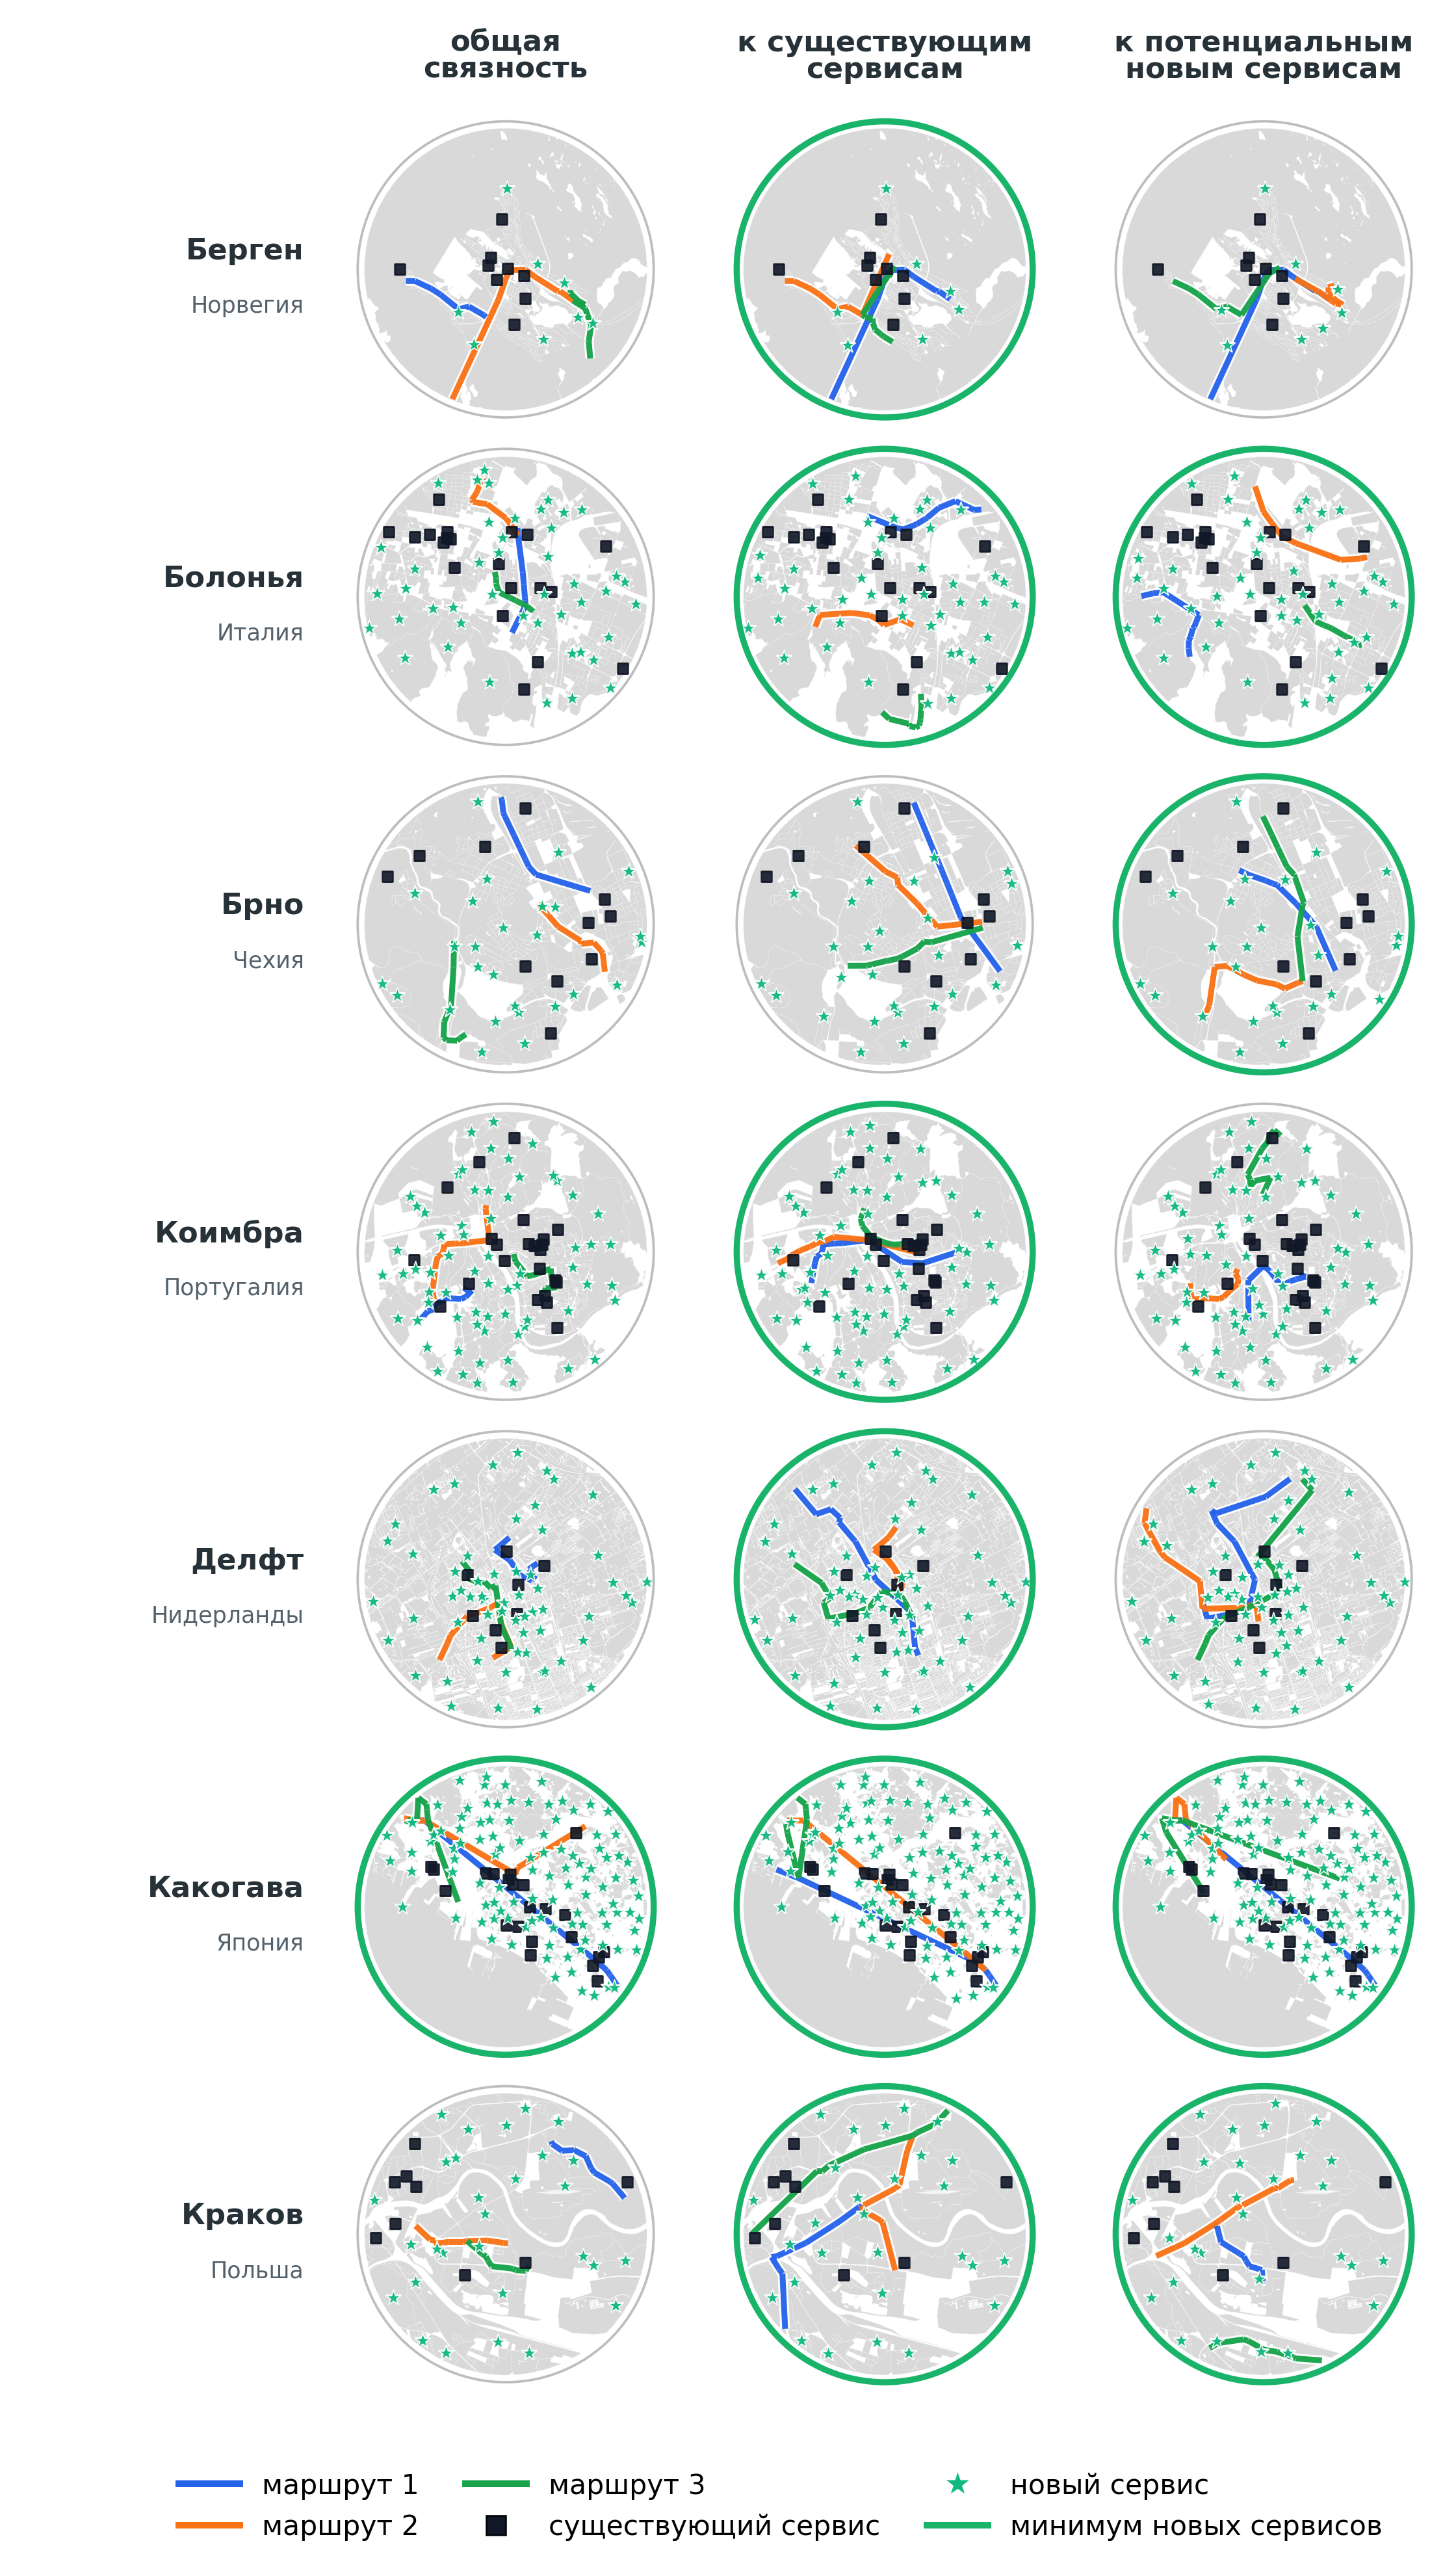
\includegraphics[width=\linewidth,height=0.82\textheight,keepaspectratio]{images/ch4/optimal_local/polyclinic_route_strategy_7x3_ru}
    \caption{Сравнение трех стратегий генерации маршрутов общественного транспорта для снижения потребности в новых поликлиниках. Зеленая рамка отмечает сценарий с минимальным числом новых объектов обслуживания.}
    \label{fig:chapter4-polyclinic-route-strategy-scenarios-expanded}
\end{figure}

\end{document}
